\documentclass[./main.tex]{subfiles}
\graphicspath{{\subfix{./figs}}}

% ------------ main document ------------ 
\begin{document}

\chapter{\chapHydro} \label{chap:hydrology}

% custom paragraph skip
\setlength{\parskip}{0mm}

\epigraph{\small{Lorem ipsum dolor sit amet consectetur adipiscing elit. Sed ac bibendum orci. Cras erat elit, consequat vel erat ac, tincidunt pulvinar lacus. Pellentesque vitae consectetur quam. Interdum et malesuada fames ac ante ipsum primis in faucibus. The typesetting markup language is specially suitable for documents that include.}}{Name (Year, p. n) [>>cite]}

\epigraph{\small{Lorem ipsum dolor sit amet consectetur adipiscing elit. Sed ac bibendum orci. Cras erat elit, consequat vel erat ac, tincidunt pulvinar lacus. Pellentesque vitae consectetur quam. Interdum et malesuada fames ac ante ipsum primis in faucibus.}}{Name (Year, p. n) [>>cite]}

% custom paragraph skip
\setlength{\parskip}{\myparskip}

\section{Bacias de ordem zero} \label{sec:hydro:intro}

\par A \textbf{\gls{hydrology}} é a ciência que estuda as águas continentais, buscando entender como a água se distribui nos continentes depois de se precipitar da atmosfera e antes de retornar aos oceanos \cite{chow1964}. Em outras palavras, a \gls{hydrology} investiga como o \textbf{\gls{hydro_cicle}} se manifesta em sua fase terrestre, em contraste com a Meteorologia (que se foca na atmosfera) ou Oceanologia (que estuda os oceanos). Ao ponderar sobre isso, é fácil imaginar grandes rios, como o Amazonas e o Paraná, além de outros notáveis como o Danúbio, o Nilo, o Amarelo, o Indo, o Ganges e o Mississípi. No caso do Brasil, surgem imagens de uma natureza exuberante, incluindo as vastas várzeas amazônicas e pantaneiras, assim como as espetaculares cataratas do rio Iguaçu. Também emergem visões relacionadas à intervenção humana em larga escala, como o complexo hidrelétrico, com suas barragens espalhadas pelo País, e os grandes projetos de transposição e irrigação, exemplificados pelos reservatórios na Serra da Cantareira, a transposição do Rio São Francisco e os pivôs centrais na bacia do Rio São Marcos. As recentes inundações que devastaram as cidades localizadas nos vales fluviais do Rio Grande do Sul, ilustram também que os rios são cruciais não somente para a produção de energia e de alimentos, mas também para a garantia da saúde básica e segurança física dos habitantes de vastas metrópoles urbanas. Nessa linha, não é raro que livros didáticos de \gls{hydrology} mencionem como as primeiras cidades-estado, surgidas na Mesopotâmia e no Egito, desenvolveram uma relação quase que simbiótica com grandes rios e suas planícies inundáveis \sethlcolor{pink}\hl{[todo:cite]}. Água e sociedade estão intimamente ligadas. 

\begin{figure}[t!] 
\centering				
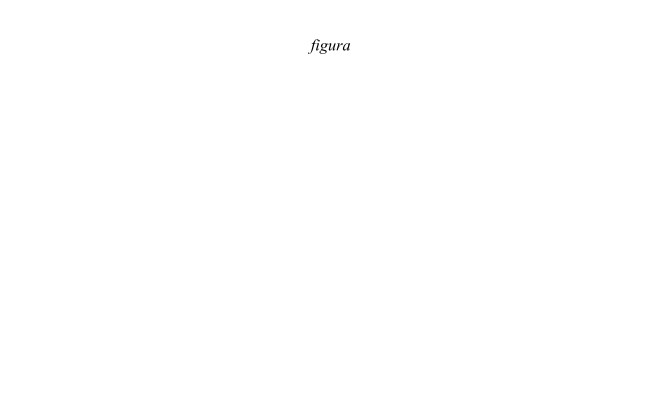
\includegraphics[width=0.95\linewidth]{figs/fig_m.jpg}		
\caption[Lorem ipsum dolor sit amet]
{\textbf{---\;Lorem ipsum dolor sit amet.}
    Lorem ipsum dolor sit amet consectetur adipiscing elit. Sed ac bibendum orci. Cras erat elit, consequat vel erat ac, tincidunt pulvinar lacus. \;\textbf{a}\;---\;Sed ac bibendum orci. Cras erat elit, consequat vel erat ac, tincidunt pulvinar lacus. Pellentesque vitae consectetur quam. Interdum et malesuada fames ac ante ipsum primis in faucibus.\;\textbf{b}\;---\;Sed ac bibendum orci. Cras erat elit, consequat vel erat ac, tincidunt pulvinar lacus. Pellentesque vitae consectetur quam. Interdum et malesuada fames ac ante ipsum primis in faucibus. \;\textbf{c}\;---\;Sed ac bibendum orci. Cras erat elit, consequat vel erat ac, tincidunt pulvinar lacus. Pellentesque vitae consectetur quam. Interdum et malesuada fames ac ante ipsum primis in faucibus.
}
\label{fig:hydro:intro} 		
\end{figure}

\par Essa interpretação intuitiva da \gls{hydrology}, no entanto, resulta de duas percepções particulares. A primeira delas é o \textbf{\gls{bias-engineer}} que permeia a \gls{hydrology}, que desde sempre é marcada por uma \textbf{\gls{dual-sci-mgmt}}. Essa dualidade implica que a \gls{hydrology} existe em uma interface fluida entre a investigação teórica sobre a natureza (problemas \textit{importantes} para o conhecimento humano) e a solução prática de impasses sociais, ambientais e econômicos (problemas \textit{urgentes} para as pessoas). James Dooge (1988) \cite{Dooge1988} sustenta que o campo nasceu de forma relativamente distinta de outras disciplinas científicas, como a Física ou Biologia, sendo essencialmente pragmática em sua formação. Ao longo da História, os problemas hidrológicos em geral se apresentavam diretamente de sua aplicação, para então novos dados serem obtidos e, por fim, algum conhecimento ser produzido. Como exemplo, Dooge ilustra que, de acordo com Plínio O Velho (24-79 DC), o nível do Rio Nilo era medido na Antiguidade não em termos de vazão, mas em uma escala do impacto socioeconômico implicado: fome (nível baixo), segurança (nível médio) e desastre (acima da cota de inundação). Nessa linha, Murugesu Sivapalan e Günter Blösch sugerem que o campo evoluiu de uma fase baseada em métodos de engenharia reducionistas e pragmáticos (Era Empírica), para tornar-se durante o século XX uma Ciência da Terra (Era da Geociência), holística e integradora, fundindo-se com ramos importantes da Geografia Física, Geologia, Pedologia, Ecologia e, recentemente, da Sociologia (Era da Co-evolução) \cite{Sivapalan2017, Sivapalan2018}. A segunda distorção é o \textbf{\gls{bias-fluvial}} que domina o campo, em especial em lugares atravessados por grandes rios, como é o caso do Brasil, dos Estados Unidos, da China e da Europa Central. Essa visão direciona os estudos hidrológicos para problemas essencialmente hidráulicos em escala continental, tais como a propagação de vazão nos canais da rede de drenagem, a inundação das planícies adjacentes e, com o advento do sensoriamento remoto, do balanço hídrico continental. A eficiência de atividades econômicas como a produção de energia elétrica, navegação, saneamento básico, irrigação, etc, dependem fundamentalmente desse tipo e conhecimento. Esse viés faz sentido em boa parte dos continentes, mas possui um peso menor em regiões dominadas por rios de pequeno e médio porte, como nos arquipélagos do Japão, da Nova Zelândia e nas Ilhas Britânicas. A perspectiva fluvialista é ilustrada pela impressão relatada por um hidrólogo brasileiro em uma visita ao Reino Unido:

\begin{adjustwidth}{100pt}{0pt}
\medskip
\small Quando eu estava na Inglaterra, fui conhecer uma certa estação fluviométrica de referência em um rio famoso na região. Falavam do tal rio o tempo todo, mas quando cheguei no local, fiquei um tanto perplexo e decepcionado. Aquilo não era um rio: era uma sanga. Com algum impulso, era possível até mesmo pular na outra margem. -- Walter Collischonn (2023, em comunicação pessoal).
\medskip
\end{adjustwidth}

\noindent Com a ação desses dois vieses, é um tanto fácil esquecer de que a água só escoa nos rios como consequência dos processos que ocorrem nas encostas dos morros e, em última instância, no perfil vertical que começa no dossel da vegetação, passa pela superfície e horizontes do solo e termina no embasamento subterrâneo de rocha. A propagação do escoamento pelos canais e as inundações de planícies nada mais são que processos de transporte e dissipação das enchentes produzidas pela interação das chuvas com o terreno mais alto e montanhoso da paisagem. Essa importância da \textit{escala da encosta} foi ressaltada inicialmente no Japão por Tsukamoto (1973) \cite{tsukamoto1973} no início dos anos 70, que ampliou a hierarquização sistemática de canais proposta por Strahler (1957) \cite{strahler1957} ao introduzir o conceito de \textbf{\gls{zero-basin}} (em japonês: \begin{CJK}{UTF8}{min}0 次 谷\end{CJK}). Ainda que a ênfase de Tsukamoto nas encostas e talvegues do terreno avance sobre questões específicas de erosão e produção de sedimentos, é evidente a sua importância primordial no \gls{hydro_cicle}. Ou seja, \textit{é nas bacias de ordem zero onde tudo começa}. Nessa mesma linha, Mediondo \& Tucci (1997) \cite{mediondo1997} utilizam o termo \textbf{bacia de vertente}, que eles também defendem ser o ponto de partida para entender a diversidade de processos hidrológicos, com reflexos tanto na micro quanto na macroescala. Utilizarei aqui o termo \gls{zero-basin}, considerando que, de acordo com Godoy \textit{et al.} (2021) \cite{godoy2021}, esse termo se popularizou na literatura internacional.

\par Ainda que a diversidade de processos nas encostas e talvegues do terreno seja importante na \gls{teoria}, isso é relevante \textit{na prática}? Ao se considerar a aplicação de modelos hidrológicos para ajudar na tomada de decisão e formulação de estratégias de alavancagem, o quanto a complexidade que existe nas bacias de ordem zero pode ser simplificada ou mesmo negligenciada? Afinal, como vimos no Capítulo \ref{chap:systems}, a modelagem de sistemas precisa fazer uso de idealizações, que são simplificações deliberadas para tornar o \gls{sys-target} mais palpável. Além disso, diante de rios que percorrem distâncias continentais, os detalhes mínimos sobre os processos hidrológicos nas bacias de ordem zero acabam por perder qualquer sentido prático. A mera confluência de dois rios de médio porte ou uma inundação de planície pode apagar completamente a assinatura hidrológica deixada por alguma característica típica produzida pelos processos nas encostas. A massa de água e de sedimentos, energia e momento necessariamente se preservam pelas leis da conservação, mas informações detalhadas são progressivamente atenuadas e misturadas no grande caudal que se desloca para o oceano. Nesse sentido, desde que um \gls{model} apresente resultados quantitativos empiricamente adequados, os detalhes sobre os processos nas bacias de ordem zero seriam irrelevantes.

\par  Esse \textit{apelo para a simplificação} torna-se uma objeção sedutora, pois facilita em grande medida o processo de modelagem. Mas ele é apenas um reflexo do \gls{bias-fluvial}: uma perspectiva que enquadra questões a serem compreendidas e problemas a serem resolvidos de montante para jusante, rio abaixo. Nessa linha, os modelos hidrológicos mais populares, ao menos no Brasil, como \texttt{SWAT}, \texttt{HEC-HMS}, \texttt{MGB}, \texttt{SWMM}, tratam as bacias de ordem zero como unidades herméticas, ou caixas-pretas, sendo impossível recuperar detalhes sobre os processos hidrológicos nas encostas e talvegues do terreno, a não ser em termos médios e agregados. No final das simulações computacionais, a visualização mais informativa possível é um mosaico de sub-bacias\footnote{Também é possível recuperar informações nas unidades de \gls{hydro-response} internas a cada sub-bacia. No entanto, como veremos adiante, essa representação é irremediavelmente estática, ao passo que os processos na escala de bacias de ordem zero são dinâmicos no tempo e no espaço.}. É claro que essa simplificação se justifica quando o objetivo de um dado estudo é compreender fenômenos e resolver problemas hidrológicos de jusante, ou seja, fluviais. Porém, para endereçar boa parte dos problemas relacionados com a segurança hídrica, como a revitalização de bacias hidrográficas, é necessário assumir um olhar de jusante para montante, encosta acima, representando com detalhes suficientes as bacias de ordem zero, pois é nessa escala que os processos relevantes acontecem e ações precisam ser especificadas. Para tanto, um \gls{model} útil deve levar suficientemente a sério o que as teorias hidrológicas dizem sobre a geração de escoamento em bacias de ordem zero. Do contrário, corre-se o risco de se instanciar um \gls{model} que não passa tanto no teste da adequação da fronteira quanto no teste da adequação da estrutura (ver Seção \ref{sec:sys:diags}). 

\par Dito isso, este capítulo marca o ponto em que passarei a articular como as teorias sobre as respostas hidrológicas em bacias de ordem zero podem ser veiculadas por modelos hidrológicos. Esse é um ponto crítico, pois aqui encontraremos todos os desafios e problemas filosóficos, científicos e técnicos expostos nos dois capítulos anteriores, mas agora sob um enfoque hidrológico. Os tópicos serão todos revisitados direta ou indiretamente, tais como a ascensão e queda de paradigmas, a refutação e confirmação de hipóteses, os problemas de estrutura, dimensionalidade e subdeterminação, etc. Em essência, se verá que a complexidade dos processos hidrológicos no solo e nas encostas trazidas por evidências empíricas, somada com a dificuldade de se obter observações diretas em uma bacia qualquer, torna qualquer tentativa de modelagem alicerçada em formalizações matemáticas contínuas e distribuídas no espaço um esforço desproporcional. Como veremos, uma solução unificadora para esse problema, proposta recentemente por Jeffrey McDonnell (2021) \cite{mcdonnell2021}, consiste em adotar modelos conceituais que representam \textit{efetivamente} os processos de \textbf{conectividade} na escala que precisamos endereçar para responder nossas perguntas de pesquisa. Voltando à \gls{analogy} da paisagem que introduzi no início desta tese, claramente estamos saindo dos vales estreitos de assuntos abstratos e filosóficos para adentrar em um campo mais aberto, de questões mais tangíveis e aplicadas. Aqui, os riachos das montanhas se unem, formando rios caudalosos que fluem por barras e barrancas.

\section{Infiltração} \label{sec:hydro:mechs}

\marginpar{
\tiny\raggedright\sffamily 
% todo
Falta articular a Figura. Fotos, \gls{percept-model} esquemático.
}

\par Na Seção \ref{sec:systems:model} do capítulo anterior, organizei um protótipo de \gls{model} hidrológico objetivando ilustrar e articular como que a \gls{sys-dyn} pode ser empregada no processo de modelagem. O \gls{concept-model} obtido, mantido em uma condição minimalista, foi construído principalmente com base na percepção de que uma bacia hidrográfica apresenta \textbf{respostas rápidas e lentas} diante dos eventos de chuva, produzindo assim o fenômeno da alternância entre as \textbf{enchentes} e as \textbf{estiagens} nos rios \cite{Hewlett1967}. Essa é uma percepção fundamental na \gls{hydrology}: quando chove, os rios ficam agitados, a água fica mais turva, os níveis sobem (resposta rápida); entre uma chuva e outra, os rios se acalmam, a água fica mais limpa, os níveis descem (resposta lenta); se demorar muito tempo para chover de novo, os riachos menores começam a secar (o \gls{system} tende a se esvaziar). Com algum rigor empírico, esse fenômeno em uma bacia hidrográfica qualquer pode ser medido e reproduzido em gráficos com o suporte de um pluviômetro e uma régua de nível. Com um pouco mais de rigor empírico, a percepção desse fenômeno fica mais apurada ao se fazer expedições de campo, observando a dinâmica espacial e temporal das nascentes e charcos (de onde a água subterrânea aflora lentamente) e das enxurradas rápidas (causadas pelas chuvas mais intensas). 

\par No contexto de bacias de ordem zero, a \gls{teoria} científica dominante hoje postula que as respostas hidrológicas aos eventos de chuva são a consequência de \textbf{múltiplos mecanismos de geração de escoamento}, superficiais e subterrâneos, tanto rápidos quanto lentos, simultâneos ou não, que serão descritos na próxima seção. Esses mecanismos foram revelados e corroborados por sucessivas investigações experimentais em pequenas bacias, encostas com trincheiras e parcelas de solo durante uma revolução científica na \gls{hydrology}, que ocorreu ao longo da segunda metade do século XX. Antes dessa revolução, contudo, a explicação científica hegemônica para as respostas rápidas e lentas das encostas era baseada principalmente na \gls{teoria} hidrológica de Robert Horton (1875-1945) \cite{Horton1933, Beven2004a}. Uma vez publicado, o \gls{percept-model} descrito por Horton consolidou-se como um verdadeiro \gls{paradigma} nos anos e décadas subsequentes, demarcando a chamada \textbf{\gls{age_inf}} -- um longo período de \gls{ciencia-normal} em que a \gls{comunidade-cientifica} desenvolveu pesquisas em frentes puras e aplicadas para articular as suas implicações \cite{Cook1946, Beven2021b}. Ainda que finalmente suplantada por uma explicação mais complexa, a \gls{teoria} de Horton, por ser científica (isto é, falseável), contribuiu sobremaneira em elevar a \gls{hydrology} de sua Era Empírica, focada em aplicações de engenharia, para ser entendida como uma Geociência, focada em explicar os fenômenos da natureza.

\begin{figure}[t!] 
\centering				

\includegraphics[width=0.95\linewidth]{figs/fig_g.jpg}		
\caption[Lorem ipsum dolor sit amet]
{\textbf{---\;Lorem ipsum dolor sit amet.}
    Lorem ipsum dolor sit amet consectetur adipiscing elit. Sed ac bibendum orci. Cras erat elit, consequat vel erat ac, tincidunt pulvinar lacus. \;\textbf{a}\;---\;Sed ac bibendum orci. Cras erat elit, consequat vel erat ac, tincidunt pulvinar lacus. Pellentesque vitae consectetur quam. Interdum et malesuada fames ac ante ipsum primis in faucibus.\;\textbf{b}\;---\;Sed ac bibendum orci. Cras erat elit, consequat vel erat ac, tincidunt pulvinar lacus. Pellentesque vitae consectetur quam. Interdum et malesuada fames ac ante ipsum primis in faucibus. \;\textbf{c}\;---\;Sed ac bibendum orci. Cras erat elit, consequat vel erat ac, tincidunt pulvinar lacus. Pellentesque vitae consectetur quam. Interdum et malesuada fames ac ante ipsum primis in faucibus.
}
\label{fig:hydro:horton} 		
\end{figure}

\par A ideia central do \gls{percept-model} de Horton é estabelecida no artigo \textit{O papel da infiltração no ciclo hidrológico}\footnote{Tradução livre de: \textit{The role of infiltration in the hydrological cycle}} (1933) \cite{Horton1933}, em que o solo é concebido como uma \textit{superfície separadora} da chuva: uma parte da água da chuva se infiltra nas encostas, alojando-se na matriz do solo, e outra parte escoa superficialmente, causando aumentos dramáticos na vazão dos rios, morro abaixo. A infiltração, assim, consistiria no processo-chave para se compreender o \gls{hydro_cicle} na sua fase terrestre:

\begin{adjustwidth}{100pt}{0pt}
\medskip
\small A infiltração divide a precipitação em duas partes, que posteriormente seguem caminhos diferentes através do \gls{hydro_cicle}. Uma parte segue através do \gls{sf-runoff} e dos canais dos rios até o oceano como escoamento fluvial; a outra parte vai inicialmente para o solo e daí através do fluxo de água subterrânea novamente para o rio ou é devolvida para o ar por processos evaporativos. Portanto, o solo atua como uma superfície separadora, e o autor acredita que vários problemas hidrológicos são simplificados ao começar por essa superfície e seguir o curso subsequente de cada parte da precipitação assim dividida, separadamente.\footnote{Tradução livre de: \textit{Infiltration divides rainfall into two parts, which thereafter pursue different courses through the hydrologic cycle. One part goes via overland flow and stream-channels to the sea as surface-runoff; the other goes initially into the soil and thence through ground-water flow again to the stream or else is returned to the air by evaporative processes. The soil therefore acts as a separating surface, and the author believes that various hydrologic problems are simplified by starting at this surface and pursuing the subsequent course of each part of the rainfall as so divided, separately.}} -- Robert Horton (1933, p. 446–447) \cite{Horton1933}. 
\medskip
\end{adjustwidth}

\par Para articular esse \gls{percept-model}, Horton instancia diversos fluxos, reservatórios e \gls{parameters} importantes do \gls{system} que representa a \gls{zero-basin}. O fluxo primordial consiste na \textbf{\gls{ground-rain}}\footnote{Tradução livre de \textit{ground-rainfall.}} , ou seja, o fluxo de chuva que de fato atinge o solo após a \textbf{\gls{interception}} da chuva total no dossel aéreo da vegetação. O solo, por sua vez, consiste em uma matriz porosa que pode armazenar água na \textbf{\gls{unsat-zone}}\footnote{Tradução livre de \textit{unsaturated zone}.}, em filmes de água mantidos pela tensão superficial de suas partículas. A acreção de água nos filmes nessa zona ocorre até um certo limite, que é a \textbf{\gls{fmc}} característica do solo\footnote{Tradução livre de \textit{field moisture-capacity}}. Horton denomina a quantidade máxima de água armazenável pela capilaridade no solo em dado momento de \textbf{\gls{fmd}}\footnote{Tradução livre de \textit{field moisture-deficiency}.}. Além desse limite, os filmes de água nas partículas começam a se mesclar e toda água adicional que se infiltra na matriz do solo percola verticalmente através dos poros pela ação da gravidade, criando uma \textbf{\gls{sat-zone}} sobre o embasamento mais profundo de rocha impermeável (ou seja, forma um aquífero livre). Horton denomina de \textbf{\gls{qv}}\footnote{Tradução livre de \textit{re-charge}.} o fluxo vertical de água da \gls{unsat-zone} para a \gls{sat-zone}, processo que pode eventualmente aumentar o nível do lençol freático (aumentando, portanto, a carga hidráulica nesse \gls{system} poroso).

\par Nesse ponto, Horton apresenta um parâmetro crucial em seu \gls{percept-model}: a \textbf{\gls{infmax}} $f$, isto é, o \gls{flux-max} possível de infiltração que a superfície do solo oferece em um dado momento. É importante destacar que essa capacidade é um atributo da fina camada superficial do solo e, de acordo com Horton, tende a ser inferior à \textbf{capacidade de transmissão} vertical de água verificada na matriz do solo, funcionando como um fator limitante crítico no \gls{system}. Dessa forma, a água de uma \gls{ground-rain} com intensidade menor ou igual à \gls{infmax} é completamente absorvida pela matriz do solo. Por outro lado, quando uma \gls{ground-rain} apresenta intensidade maior que a \gls{infmax}, então a água da \textbf{\gls{ex-rain}}\footnote{Tradução livre de \textit{rainfall-excess}.}passa a preencher as pequenas depressões superficiais. Se a \gls{ex-rain} persistir por tempo suficiente, a \textbf{\gls{sfmax}}\footnote{Tradução livre de \textit{detention-storage}.} é superada, e então se inicia o processo de \textbf{\gls{rie}}\footnote{Essa nomenclatura objetiva evitar confusões futuras, ainda que o termo original de Horton seja simplesmente \say{escoamento superficial} (\textit{surface-runoff}).}, onde a água da chuva escoa pelos sulcos e ravinas morro abaixo até atingir os canais dos riachos. 

\par A \gls{infmax} depende do tipo de solo, de sua textura e das práticas de manejo empregadas, o que implica em uma variabilidade na resposta de diferentes bacias, mesmo quando submetidas a eventos de chuva idênticos. Além da variabilidade espacial, Horton argumenta que a \gls{infmax} do solo varia ao longo do tempo, oscilando dinamicamente entre extremos da capacidade mínima e máxima, em um \textbf{ciclo de decaimento e restauração}. Nesse ciclo, a fase de decaimento ocorre durante os eventos de chuva em função da expansão de partículas coloidais, da colmatação por partículas finas e da compactação causada pelo impacto das gotas de chuva. Por outro lado, a fase de restauração ocorre durante os períodos de tempo seco, à medida que se abrem novas fissuras e poros pela retração das partículas coloidais, dilatações por diferenças de temperatura e pela atividade da fauna do solo, como insetos e minhocas. Com essa concepção, espera-se que uma chuva longa, mesmo que de relativa baixa intensidade, eventualmente produza \gls{sf-runoff} se o decaimento em curso levar a \gls{infmax} do solo para um valor \textit{abaixo} da intensidade da \gls{ground-rain}. Além disso, esse conceito introduz o efeito das \textbf{\gls{amc}}, como a diferença nas respostas entre o início e o final de uma estação chuvosa ou durante a entrada de uma frente fria com chuvas persistentes. Nesse caso, e se a velocidade de restauração da \gls{infmax} do solo for relativamente lenta, as chuvas subsequentes, mesmo que \textit{menos} intensas, tendem a produzir \textit{mais} \gls{sf-runoff} do que as chuvas iniciais. Em outras palavras, o comportamento do \gls{system} torna-se altamente não-linear.

\par Com a \gls{teoria} sobre o papel da infiltração no \gls{hydro_cicle}, Horton então avança para explicar definitivamente o fenômeno das enchentes\footnote{Tradução livre de \textit{stream rises}.} observada nos rios, propondo um método de separação do hidrograma. Com esse objetivo, ele sustenta que o escoamento fluvial\footnote{Tradução livre de \textit{total runoff}.} consiste em duas componentes de fluxo separáveis: (1) o fluxo de água subterrânea\footnote{Tradução livre de \textit{ground-water runoff}.}, que é uma resposta lenta do afloramento do aquífero livre, e; (2) o fluxo do escoamento superficial\footnote{Tradução livre de \textit{surface-runoff}.}, que é uma resposta rápida das enxurradas produzidas nas encostas. As duas respostas são controladas, em todo ou em parte, pela \gls{infmax} do solo:

\begin{adjustwidth}{100pt}{0pt}
\medskip
\small De acordo com esta \gls{teoria}, o escoamento fluvial total consiste em duas partes: (1) Escoamento superficial, que depende da quantidade de precipitação, da intensidade da chuva e da \gls{infmax} e é praticamente independente da taxa de evaporação. (2) Escoamento de água subterrânea. Este depende de (a) infiltração total e, portanto, indiretamente dos mesmos fatores que controlam o \gls{sf-runoff} e também depende de (b) atividade vegetal e evaporação, que em parte determinam as perdas de água, e de (c) as complexas inter-relações entre \gls{infmax}, \gls{fmc} do solo, atividade vegetal e \gls{qv} do aquífero.\footnote{Tradução livre de: \textit{In accordance with this theory, total runoff consists of two parts: (1) Suface-runoff, which is dependent on rainfall-amount, rain-intensity, and infiltration-capacity and is practically independent of evaporation-rate. (2) Ground-water runoff. This is dependent on (a) total infiltration and hence indirecty on the same factors which control surface-runoff and is also dependent on (b) vegetational activity and evaporation, which in part determine the water losses, and on (c) the complex interrelations between infiltration-capacity, field moisture-capacity, vegetational activity, and accretion to the water-table.}} -- Robert Horton (1933, p. 454) \cite{Horton1933}.
\medskip
\end{adjustwidth}

\noindent Assumindo que o aquífero livre funciona como um \gls{linear-reserv}, a \textbf{\gls{deple-curve}}\footnote{Tradução livre de \textit{normal depletion curve}.} do fluxo de afloramento da água subterrânea consiste em uma típica \gls{curve-exp-dec} do tipo $q = q_o e^{-c t}$. Essa curva é uma característica física constante do aquífero e pode ser extraída de hidrogramas durante os períodos de estiagem nos quais as perdas de água do aquífero por evapotranspiração são mínimas (por exemplo, nos meses mais frios em locais de clima temperado e subtropicais). Uma vez obtida, a \gls{deple-curve} pode ser deslocada horizontalmente no hidrograma, permitindo-se separar a componente superficial da vazão fluvial da contribuição puramente subterrânea. Com isso, Horton propõe que existem quatro  tipologias possíveis de \gls{hydro-response} diante dos eventos de chuva. A resposta \textbf{Tipo 0} ocorre quando a intensidade da \gls{ground-rain} é inferior à \gls{infmax} e o total de água infiltrada é inferior ao déficit de campo (\textit{não} há \gls{sf-runoff} e \textit{não} há recarga). Nessa situação, mesmo que tenha chovido, não há mudança detectável na curva de recessão do rio. A resposta \textbf{Tipo 1}, por sua vez, ocorre quando a intensidade da \gls{ground-rain} é inferior à \gls{infmax}, mas o total de água infiltrada é superior ao déficit de campo (\textit{não} há \gls{sf-runoff} mas \textit{ocorre} \gls{qv} do aquífero). Nesse caso, a curva de recessão é deslocada, dependendo de quanto a \gls{qv} é superior (ou inferior) ao fluxo de afloramento, podendo inclusive produzir um pulso (relativamente lento) na vazão do rio puramente pelo aumento da carga hidráulica no \gls{system} aquífero. A resposta \textbf{Tipo 2} ocorre quando a intensidade da \gls{ground-rain} é superior à \gls{infmax} e o total infiltrado é muito baixo, inferior ao déficit de campo (\textit{ocorre} \gls{sf-runoff} mas \textit{não} ocorre \gls{qv} do aquífero). Esse tipo de resposta consiste em um pulso rápido de água da enxurrada superficial sobreposto à curva de recessão que se desenvolvia antes do evento. Por fim, a resposta \textbf{Tipo 3} acontece quando as duas respostas, rápida e lenta, ocorrem simultaneamente: tanto o \gls{sf-runoff} quanto a \gls{qv} do aquífero se manifestam na forma de pulsos sobrepostos. Essas quatro tipologias ilustram a complexidade que emerge a partir do \gls{percept-model} de Horton, proporcionando grande margem para explicações sobre as enchentes, que variam de acordo com as características da superfície, do solo, do subsolo, das chuvas e das condições antecedentes de umidade.

\par Diante desse \gls{percept-model}, diversos modelos conceituais foram então desenvolvidos por abordagens físicas (quando princípios físicos são aplicados \textit{a priori}) e empíricas (quando equações são ajustadas aos dados \textit{a posteriori})  \cite{mishra2003}. Na linha da abordagem física, destacam-se os avanços de Philip (1957) \cite{philip1957}, que arquitetou os fundamentos de uma \gls{teoria} matematicamente formal da infiltração como um caso especial da equação de Darcy-Richards, ou seja, do movimento da água em um meio poroso não saturado. Pelo lado empírico, o próprio Robert Horton manteve uma linha de pesquisa aplicada, propondo um \gls{concept-model} de decaimento exponencial para a \gls{infmax} do solo \cite{Horton1939}. Com isso, a produção de curvas de infiltração padronizadas experimentalmente viabilizou uma técnica mais sofisticada para se estimar o total de \gls{sf-runoff}, em contraste com o \textbf{Método Racional}, que é baseado em um simples coeficiente de escoamento \cite{Cook1946}. Outro método empírico de grande influência prática produzido nesse contexto foi o \textbf{\gls{cn_method}}, que foi desenvolvido pelo \acrfull{scs}\footnote{Atual \acrfull{usda}} em 1954 e apresentado como uma diretriz técnica nas décadas seguintes. De acordo com Rallison \& Miller (1981) \cite{Rallison1981}, o método \acrshort{cn} do \acrshort{cn} surgiu levando em conta os resultados de pesquisas experimentais em pequenas bacias, mas foi principalmente motivado pela aprovação de uma legislação de proteção ambiental nos Estados Unidos. Consta que Horton foi consultor do \acrshort{scs}, mas o seu método das curvas de infiltração não teve muito sucesso, cedendo lugar à abordagem agregada de Mockus (1949) \cite{mockus1949}, que avalia a relação entre os totais de chuva e escoamento para eventos individuais. Justificada por essas evidências, a equação do Método CN\footnote{A equação do método \acrshort{scs} é dada por: $R = \frac{(P - I_a)^{2}}{(P - I_a + S)}$, em que $R$ (mm) é o \gls{sf-runoff} total, equivalente à \gls{ex-rain}; $P$ é a chuva total (mm); $S$ (mm) é a \gls{sfmax}, calculada pelo parâmetro CN: $S = \frac{1000}{\text{CN}}-10$, e; $I_a$ (mm) são as abstrações iniciais (incluindo infiltração e interceptação), calculada ao se assumir que $I_a = 0.2S$. De acordo com Rallison \& Miller (1981) \cite{Rallison1981}, a equação emerge do balaço hídrico da \gls{ground-rain} e segundo a premissa de que a razão entre \gls{sf-runoff} ($Q$) e \gls{ground-rain} ($P - I_a$) é a mesma que a razão entre a detenção superficial ($F$) e a capacidade de detenção ($S$), ou seja: $Q/(P-I_a) = F/S$. Talvez o método \acrshort{cn} pareça menos arbitrário se os dados de Mockus e Sherman forem interpretados como a marca de um \textit{processo de saturação} superficial, o que resulta em uma equação homóloga.} busca expressar a suposta \textit{transição} de uma resposta \textit{não-linear} (quando a infiltração e detenção superficial dominam o balanço de água superficial) para uma resposta \textit{linear} (quando a intensidade da \gls{ground-rain} é superior à \gls{infmax} e detenção superficial). O parâmetro CN, nesse sentido, calibra o efeito da não-linearidade para diferentes tipos de solo, coberturas, práticas de manejo e condições antecedentes de umidade. Rallison \& Miller apontam que a escolha dessa abordagem pelo \acrshort{scs} teve um forte viés de conveniência, pois os dados utilizados estavam prontamente disponíveis em escala nacional (nos Estados Unidos). Não obstante, a essência do método \acrshort{cn} reproduz o \gls{percept-model} de Horton, pois o \gls{sf-runoff} é tido como a única resposta rápida da bacia hidrográfica e é determinado pela estimativa da \gls{ex-rain}. 

\section{Diferenciação}

\marginpar{
\tiny\raggedright\sffamily 
Falta articular a Figura. Apresentar a visão geral, usar Kirkby, Dunne, McDonnell
}

\par Na Seção \ref{sec:epis:kuhn} ressaltei que, segundo Thomas Kuhn, o sucesso de uma \gls{teoria} científica está principalmente associado com a sua \textit{competitividade} em relação a outras ideias que circulam pela \gls{comunidade-cientifica}. Assim, uma \gls{teoria} tende a se estabelecer como o \gls{paradigma} hegemônico quando ela é eficiente tanto em explicar os fenômenos conhecidos quanto em abrir frentes de investigação promissoras para as novas gerações de pesquisadores. Na ausência de teorias concorrentes estruturadas nesse sentido, o \gls{percept-model} de Horton para explicar as respostas hidrológicas rápidas e lentas entregou esses dois atributos para uma \gls{comunidade-cientifica} fortemente marcada pelo \gls{bias-engineer} e pelo \gls{bias-fluvial}. Essas duas características possuem um efeito de blindar as percepções que tecnicamente são irrelevantes para solucionar os típicos problemas de jusante, pois não precisam dos detalhes sobre o que acontece nas bacias de ordem zero\footnote{Ironicamente, era exatamente esse o objetivo do \acrshort{scs} -- proteger o solo nas encostas.}. O \gls{model} Hortoniano, mesmo que parcial ou completamente incorreto, não impediu que fossem feitas boas estimativas de vazões de projeto para pontes, barragens, balanço hídrico em grandes bacias, etc. Afinal, a equifinalidade dos sistemas permite que comportamentos semelhantes se manifestem a partir de mecânicas distintas (até o dia que todos são surpreendidos). No âmbito estritamente técnico, em certa medida, o desenvolvimento do método \acrshort{cn} pelo \acrshort{scs} \textit{perpetuou} as ideias da \gls{age_inf}, sendo geralmente o método básico exigido ou aceito por diretrizes técnicas em projetos de engenharia e o principal módulo de geração de escoamento em diversos modelos hidrológicos distribuídos em \textit{softwares}, como o \texttt{SWAT} e \texttt{SWMM}\footnote{Na minha graduação como Engenheiro Ambiental fui treinado a aplicar o método racional e \acrshort{cn} para estimativa de \say{vazões de projeto}. Inclusive, durante meu intercâmbio nos Estados Unidos em 2014-2015, ganhei uma cópia impressa da \textit{Technical Release} 55 do \acrshort{usda}, que basicamente é a versão mais recente do método \acrshort{cn} aplicada em projetos de drenagem urbana nos Estados Unidos.}. 

\begin{figure}[t!] 
\centering				

\includegraphics[width=0.95\linewidth]{figs/fig_g.jpg}		
\caption[Lorem ipsum dolor sit amet]
{\textbf{---\;Lorem ipsum dolor sit amet.}
    Lorem ipsum dolor sit amet consectetur adipiscing elit. Sed ac bibendum orci. Cras erat elit, consequat vel erat ac, tincidunt pulvinar lacus. \;\textbf{a}\;---\;Sed ac bibendum orci. Cras erat elit, consequat vel erat ac, tincidunt pulvinar lacus. Pellentesque vitae consectetur quam. Interdum et malesuada fames ac ante ipsum primis in faucibus.\;\textbf{b}\;---\;Sed ac bibendum orci. Cras erat elit, consequat vel erat ac, tincidunt pulvinar lacus. Pellentesque vitae consectetur quam. Interdum et malesuada fames ac ante ipsum primis in faucibus. \;\textbf{c}\;---\;Sed ac bibendum orci. Cras erat elit, consequat vel erat ac, tincidunt pulvinar lacus. Pellentesque vitae consectetur quam. Interdum et malesuada fames ac ante ipsum primis in faucibus.
}
\label{fig:hydro:diff} 		
\end{figure}

\par Apesar de que talvez o \gls{paradigma} da infiltração tenha se consolidado simplesmente pela falta de competidores, a sua crise esteve presente desde a sua formação, nos anos 1930 e 1940. Por exemplo, os dados de intensidade de chuva e \gls{infmax} do solo medidos pelo próprio laboratório de Robert Horton sugerem que é muito \textit{improvável} que ele mesmo tenha observado \gls{sf-runoff} generalizado na sua bacia experimental em La Grange Brook (14.4 ha, Nova Iorque) \cite{Beven2004c}. Os dados do laboratório, avaliados por Keith Beven, indicam que o solo nas principais coberturas da bacia (campos e pomares) apresentava uma \gls{infmax} relativamente alta diante das chuvas registradas. Na verdade, a conciliação entre as medições feitas por Horton da \gls{infmax} do solo \textit{in situ}, o \textbf{valor de campo}, com estimativas na escala de bacia, o \textbf{valor aparente}, possivelmente nunca fizeram muito sentido entre si, exigindo numerosas \gls{aux-hyp} e \gls{neglig-premis} (o \textbf{problema da escala}, que veremos adiante). Isso ficou claro no artigo de Betson (1694) \cite{Betson1964}, que conseguiu excelentes ajustes de um \gls{concept-model} aos dados observados somente após \textit{relaxar} o \gls{model} Hortoniano, implicando um conceito \textbf{área de contribuição parcial} de escoamento superficial\footnote{Do ponto de vista racionalista, Betson tentou \say{salvar} a \gls{teoria} de Horton, admitindo modificações \textit{ad hoc} para evitar a sua refutação.}. Ainda que estatisticamente bem ajustados, os resultados insinuavam que uma fração pequena e relativamente constante nas bacias no vale do Rio Tennessee produziam \gls{sf-runoff} (bacias entre 500 ha até 8,4 km², Carolina do Norte).

\par Mas foi ao longo da década de 1960 que a \gls{age_inf} encontrou sua crise derradeira no âmbito científico. A revolução nas percepções da \gls{comunidade-cientifica} ocorreu após uma profusão de evidências empíricas acumularem-se na literatura, relatando a observação de novos mecanismos de \gls{hydro-response} das encostas, que serão descritas nas próximas seções. Podemos resumir aqui o advento de pelo menos três novos mecanismos de resposta rápida (ou potencialmente rápida) além daquele postulado por Horton: (1) \textbf{\gls{subsur_flow}}\footnote{Esse mecanismo, além do estranho nome de \say{afloramento pluvial} (\textit{storm-seepage}), também foi denominado na literatura por diversos outros títulos: fluxo de retorno (\textit{return flow}), fluxo de passagem (\textit{throughflow}), interfluxo (\textit{interflow}), fluxo lateral (\textit{lateral flow}) e \say{exfiltração} (\textit{exfiltration}).}; (2) \textbf{\gls{rse}}\footnote{Tradução livre de: \textit{saturation-excess runoff}.}, e; (3) \textbf{\gls{trans_flow}}\footnote{Tradução livre de: \textit{translational flow}.}. Os dois primeiros se referem à água nova da chuva que contribui para as enchentes. O último consiste na água velha armazenada no subsolo, que também contribui para a resposta rápida (com taxas de prevalências surpreendentes). A nomenclatura sobre esses mecanismos varia bastante ainda hoje, além do fato de muitos processos de escoamento que são observados em campo com rótulos diferentes são, no fundo, manifestações desses mecanismos mais primitivos (por exemplo, o afloramento da água em nascentes pode ser tanto uma resposta lenta quanto rápida). Em contraste com o \gls{model} Hortoniano, essas respostas rápidas incluem rotas superficiais e subterrâneas controladas por outras partes do \gls{system} além da camada superficial do solo, como a \textbf{\gls{macropor}} (caminhos preferenciais laterais e verticais no solo) e a topografia (padrões dinâmicos de saturação do solo). Em essência, as evidências empíricas na segunda metade do século XX expuseram irreversivelmente a complexidade dos processos em bacias de ordem zero.

\par Um marco para o início do fim da \gls{age_inf} foi o artigo de Mike Kirkby (1969) \cite{Kirkby1969}, que revisou resultados de diversos estudos experimentais e apresentou didaticamente uma nova forma de compreender e nomear os processos hidrológicos em bacias de ordem zero. Nesse ponto, Kirkby (1969) demarca definitivamente a importância das respostas rápidas de água que transita no solo por uma rede de macroporos (escoamento subsuperficial). Após mais de uma década de novas evidências empíricas se acumulando, um marco para a ascensão do novo \gls{paradigma} foi o artigo de Thomas Dunne (1983) \cite{Dunne1983}, que organizou definitivamente uma nova visão esquemática sobre as respostas hidrológicas, propondo um novo programa promissor de pesquisas nas frentes pura e aplicada. Dunne (1983) deixa claro a ideia de que diferentes climas, escalas e paisagens favorecem a \textit{dominância} de um ou de outro mecanismo, ainda que eles possam acontecer simultaneamente ou se alternar sazonalmente. Por exemplo, em climas semi-áridos, fatores como os longos períodos de estiagem e a formação de crostas no solo favorecem o mecanismo de Horton -- a \gls{infmax} tende a ser insuficiente e sequer existem áreas saturadas nos fundos de vale no final da estação seca. Em climas tropicais úmidos, por outro lado, a formação de solos profundos ou o excesso de água na estação chuvosa pode favorecer tanto um mecanismo quanto outro. Por fim, essa revolução produziu novos entendimentos sobre a complexa relação desses mecanismos, como demonstrado por Jeffrey McDonnell (1990) \cite{mcdonnell1990} no caso da Bacia Experimental de MaiMai (Nova Zelândia). Mas McDonnell (2013) \cite{Mcdonnell2013} também estabelece uma crítica ao \gls{paradigma} que se instalou: o programa de pesquisa hegemônico se pauta principalmente em \textit{diferenciar} as múltiplas respostas hidrológicas, reafirmando a ideia de complexidade e singularidade de cada ambiente. Ainda que essa atitude possa seguir \textit{ad infinitum}, ele argumenta que o objetivo verdadeiro de uma ciência hidrológica talvez seja o de produzir \textit{generalizações}, teorias que sejam \textit{unificadoras}. Nesse espírito, o \gls{paradigma} hidrológico vigente talvez mereça o título de \textbf{\gls{age_diff}}.

\subsection{Macroporos}

\marginpar{
\tiny\raggedright\sffamily 
Falta articular a Figura. Apresentar fotos, \gls{percept-model} esquemático
}

\par No final dos anos 1930 e início dos anos 1940, a literatura científica já reconhecia as fragilidades do \gls{model} de Horton, sustentando que a resposta rápida de pequenas bacias deveria incluir um ou mais mecanismos \textit{subterrâneos}. Snyder (1939) \cite{Snyder1939}, por exemplo, sugere o uso do termo \textit{\gls{sf-runoff} direto}\footnote{Tradução livre de \textit{direct-runoff}.} para denotar a água da chuva que contribui para a enchente do rio \textit{sem nunca ter transitado pelo solo}. Nesse contexto, Barnes (1939) \cite{Barnes1939} divide em \textit{três} (e não \textit{duas}) as componentes do escoamento fluvial\footnote{Tradução livre de \textit{stream-flow}.}: (1) escoamento superficial\footnote{Tradução livre de \textit{surface-flow}.}; (2) afloramento pluvial\footnote{Tradução livre de \textit{storm-seepage}.} e; (3) escoamento de base\footnote{Tradução livre de \textit{base-flow}.}. Por \say{afloramento pluviall} (\textit{storm-seepage}) Barnes se referia a um escoamento subterrâneo rápido da água da chuva que se move \textit{lateralmente} pela \gls{unsat-zone}, alimentando os canais dos riachos com uma velocidade muito superior ao que é esperado da capacidade de transmissão do aquífero livre:

\begin{adjustwidth}{100pt}{0pt}
\medskip
\small Isto consiste na água que penetrou apenas nas camadas superiores do solo durante uma chuva ou degelo e filtrou-se mais ou menos horizontalmente através do solo para desaguar no \gls{system} de rios por afloramentos. Esse fenômeno foi observado pelo autor em 1936 enquanto analisava os dados de vazão do Rio Zumbro em Minnesota e denominado por ele como \say{fluxo de base secundário}.\footnote{Tradução livre de: \textit{This consists of water which has penetrated only the upper soil-layers during a rainstorm or a thaw and has filtered more or less horizontally through the soil to discharge into the stream-system by seepage. It was observed by the writer in 1936 while analyzing discharge records of Zumbro River in Minnesota and called by him \say{secondary base-flow}.}} -- Bertram Barnes (1939, p. 721) \cite{Barnes1939}.
\medskip
\end{adjustwidth}

% figure
\begin{figure}[t!] 
\centering				

\includegraphics[width=0.95\linewidth]{figs/fig_p.jpg}		
\caption[Lorem ipsum dolor sit amet]
{\textbf{---\;Lorem ipsum dolor sit amet.}
    Lorem ipsum dolor sit amet consectetur adipiscing elit. Sed ac bibendum orci. Cras erat elit, consequat vel erat ac, tincidunt pulvinar lacus. \;\textbf{a}\;---\;Sed ac bibendum orci. Cras erat elit, consequat vel erat ac, tincidunt pulvinar lacus. Pellentesque vitae consectetur quam. Interdum et malesuada fames ac ante ipsum primis in faucibus.\;\textbf{b}\;---\;Sed ac bibendum orci. Cras erat elit, consequat vel erat ac, tincidunt pulvinar lacus. Pellentesque vitae consectetur quam. Interdum et malesuada fames ac ante ipsum primis in faucibus. \;\textbf{c}\;---\;Sed ac bibendum orci. Cras erat elit, consequat vel erat ac, tincidunt pulvinar lacus. Pellentesque vitae consectetur quam. Interdum et malesuada fames ac ante ipsum primis in faucibus.
}
\label{fig:hydro:macro} 		
\end{figure}

\noindent Assim, é feita uma diferença entre as \textbf{\gls{nasc_perenes}}, alimentadas pelo escoamento da água subterrânea \say{verdadeira} (aquífero livre), das \textbf{\gls{nasc_efemeras}}, alimentadas pelo \gls{subsur_flow} da água da chuva (aquífero suspenso). Esse mecanismos de resposta foi imensamente reforçado por estudos conduzidos por Charles Hursh na Floresta Experimental de Coweeta (Carolina do Norte, Estados Unidos), com resultados reportados para diversas bacias florestadas com áreas entre 16 a 760 hectares \cite{Hoover1943, Hursh1944}. Por exemplo, Hursh \& Brater (1941) \cite{Hursh1941} alegam que jamais se observou \gls{sf-runoff} nas encostas de uma das bacias monitoradas, apesar das respostas rápidas observadas na vazão do rio: 

\begin{adjustwidth}{100pt}{0pt}
\medskip
\small O escoamento das chuvas na forma de \gls{sf-runoff} não foi observado nesta área de drenagem; ainda assim, hidrogramas de enchentes característicos são produzidos por chuvas intensas.\footnote{Tradução livre de: \textit{Surface storm-runoff as overland-flow has not been observed on this drainage-area; nevertheless, characterlstlc flood-hydrographs are produced by heavy rains.}} -- Hursh \& Brater (1941, p. 863) \cite{Hursh1941}.
\medskip
\end{adjustwidth}

\noindent Essa alegação fatalmente introduz um \textit{contra-exemplo} para a \gls{teoria} da \gls{infmax}. Afinal, se não há \gls{sf-runoff}, a única resposta disponível no \gls{percept-model} de Horton é a resposta \textit{lenta} causada pela \gls{qv} do aquífero, responsável pela curva de recessão. Entre outros mecanismos em ação na bacia, detalhados mais adiante, os autores apontam a existência de respostas \textit{subterrâneas rápidas} que incluem tanto o fluxo de água em camadas de solo altamente permeáveis (fluxo não saturado), quanto a formação de aquíferos suspensos temporários (fluxo saturado), que se desenvolvem em diferentes partes da paisagem durante as chuvas. Nessa direção, Hursh \& Fletcher (1942) \cite{Hursh1942} salientam a importância da \gls{macropor} do solo. Especialmente em florestas, essa propriedade ajudaria a explicar a dominância de fluxos preferenciais subsuperficiais, aumentando tremendamente a \textbf{\gls{water_gravit}} do solo, em oposição à \textbf{\gls{water_capilar}}:

\begin{adjustwidth}{100pt}{0pt}
\medskip
\small A natureza exata deste espaço macroporoso ocorrendo em diferentes horizontes do perfil do solo ainda precisa ser descrita. Ela inclui todos os grandes canais subterrâneos formados por raízes decompostas, rochas fraturadas, túneis de insetos e animais, e espaços maiores que possam existir. Também inclui espaços macroporosos formados através dos complexos padrões estruturais criados pela agregação de partículas do solo na presença de materiais orgânicos. Nos horizontes superiores dos solos naturais, essas aberturas biológicas e padrões estruturais construídos a partir de agregados semelhantes a treliças são muito mais importantes na determinação da porosidade não capilar do que o tamanho das partículas individuais do solo. Canais de raízes e túneis de animais são particularmente significativos no armazenamento e drenagem da \gls{water_gravit}. Um único túnel de minhoca pode ser muito mais importante na drenagem de um bloco de solo maciço do que toda a área da seção transversal do espaço poroso. Da mesma forma, é concebível que alguns poucos espaços vazios contínuos possam dar origem a uma descarga rápida de água subterrânea através de um perfil de solo que, quando visto como um meio uniformemente permeável, seria esperado transmitir água lentamente.\footnote{Tradução livre de: \textit{The exact nature of this macro-pore space occurring in different horizons of the soil profile has yet to be described. It includes all large underground channels formed from decayed roots, fractured rock, insect and animal burrows, and larger spaces that may exist. It also includes macro-pore spaces formed through the complex structural patterns created by the aggregation of soil particles in the presence of organic materials. In the upper horizons of natural soils these biological openings and structural patterns built up from lattice-like aggregates are far more important in determining noncapillary porosity than the single grain soil particle size. Root channels and animal burrows are of particular significance in the detention storage and draining of gravitational water. A single earthworm burrow may be far more important in draining through a block of heavy soil than the entire cross sectional area of the pore space. In like manner, it is conceivable that a few continuous void spaces may give rise to rapid discharge of groundwater through a soil profile which, when viewed as a uniformly pervious medium, would be expected to transmit water slowly.}} -- Hursh \& Fletcher (1942, p. 485) \cite{Hursh1942}.
\medskip
\end{adjustwidth}

\par Esses autores, contudo, não apresentaram evidências quantitativas além de observações de processos agregados, como chuva, vazão e níveis de poços. Essa lacuna de pesquisa foi permanentemente solucionada nos anos 1960, quando uma nova onda de estudos trouxe resultados quantitativos mais detalhados, obtidos por uma abordagem mais experimental do que observacional. Ainda no contexto da Floresta Experimental de Coweeta, Hewlett e Hibbert (1963) \cite{Hewlett1963} usaram um lisímetro para demonstrar o papel crítico do fluxo de água na \gls{unsat-zone} em sustentar o escoamento de base dos riachos. Whipkey (1965) \cite{Whipkey1965} detalhou os fluxos laterais no perfil de solo de uma encosta em Ohio (EUA). A encosta foi monitorada por uma trincheira na sua base, demonstrando a dinâmica do \gls{subsur_flow}, especialmente nas camadas orgânicas superiores, onde foram medidas altas condutividades hidráulicas devido aos macroporos. Aqui, aparece a função exercida pelas \textbf{\gls{perm_trans}} entre os horizontes do solo, uma perda de carga hidráulica que acaba causando um fluxo \textit{lateral} na \gls{unsat-zone}. Outros estudos detalhados em trincheiras que chegaram em conclusões semelhantes nos Estados Unidos incluem: Ragan (1968), em Vermont \cite{Ragan1968}; Beasley (1976), no Mississippi \cite{Beasley1976}, e; Harr (1977), no Oregon \cite{Harr1977}. No último caso, relatou-se que o \gls{subsur_flow} foi de 6 a 9 vezes maior nas camadas superiores do solo que nas camadas inferiores, corroborando a função da \gls{macropor}. Nesse mesmo estudo, os autores relatam que o \gls{subsur_flow} foi responsável por cerca de 97\% da resposta rápida nas enchentes. Isso foi consistente com os resultados anteriores de Patric e Swanston (1968) \cite{patric1968}, que cortaram todas as árvores de uma encosta no Alasca e aplicaram irrigação por aspersão. Eles não observaram \gls{sf-runoff} -- a água aplicada percorreu caminhos subterrâneos preferenciais, aflorando rapidamente na base da encosta. Nas Ilhas Britânicas, Weyman (1970) \cite{weyman1970} reportou que o escoamento não-saturado subterrâneo consiste na principal resposta rápida em uma bacia experimental, enquanto que Jones (1971) \cite{Jones1971} fez observações de que a ocorrência generalizada do fenômeno de \textit{piping} -- a formação de túneis naturais no perfil do solo -- contribui para altas velocidades na resposta subterrânea. Consolidando essa nova geração de pesquisas de campo, os resultados a partir na bacia experimental MaiMai (Nova Zelândia) estabeleceram o novo programa de pesquisa experimental, com a aplicação combinada de balanço hídrico, trincheiras e a novidade dos traçadores químicos, corantes e isotópicos. No caso de MaiMai, Mosley (1979) \cite{Mosley1979} reafirma (quase quarenta anos depois de Hursh) o papel crucial da \gls{macropor} e túneis naturais no \gls{subsur_flow} ao rebater algumas objeções teóricas:

\begin{adjustwidth}{100pt}{0pt}
\medskip
\small Freeze [1972, p. 1282] considerou que um valor limiar de condutividade hidráulica saturada da ordem de 0,002 cm/s é necessário para que o \gls{subsur_flow} seja significativo, mas em um solo que contém canais de raízes, túneis e zonas de afloramento, a condutividade hidráulica saturada não é um fator limitante. O fluxo de corante traçador através de macroporos no solo foi observado a taxas até 3 ordens de magnitude maiores, e a resposta sensível e rápida do \gls{subsur_flow} às variações na precipitação sugere que o fluxo por macroporos, e não pela matriz do solo, contribui para as enchentes nos canais.\footnote{Tradução livre de: \textit{Freeze [1972, p. 1282] considered that a threshold value for saturated hydraulic conductivity of the order of 0,002 cm/s is necessary for subsurface stormflow to be significant, but in a soil that contains root channels, pipes, and seepage zones, saturated hydraulic conductivity is not a limiting factor. Flow of dye tracer through macropores in the soil was observed at rates up to 3 orders of magnitude greater, and the sensitive as rapid response of subsurface flow to variations in precipitation suggests that flow through macropores rather than through soil matrix contributes to channel stormflow.}} -- Paul Mosley (1979, p. 806) \cite{Mosley1979}.
\medskip
\end{adjustwidth}

\subsection{Topografia}

\marginpar{
\tiny\raggedright\sffamily 
% todo
Falta articular a Figura. Fotos, \gls{percept-model} esquemático.
}

\par O \gls{paradigma} Hortoniano não foi apenas refutado pela constatação do \gls{subsur_flow}, pois evidências empíricas também acumularam-se para sustentar a existência de mais dois mecanismos de resposta rápida, menos intuitivos, que ocorrem em \textbf{\gls{sat_areas}}. Esses mecanismos, resultam da interação da chuva com um lençol freático raso e dinâmico, sendo um o \gls{rse}, e o outro o escoamento subterrâneo translacional (detalhes na próxima seção). Ambos estão relacionados entre si, são fortemente controlados pela topografia do terreno e também produzem consequências sobre a manifestação do \gls{subsur_flow} em macroporos, como veremos adiante. O primeiro deles surge na literatura quando a precipitação direta na área do entorno de canais e nascentes é citada por Hursh \& Brater (1941) \cite{Hursh1941} como umas das fontes de escoamento fluvial nas bacias da Floresta Experimental de Coweeta:   

\begin{adjustwidth}{100pt}{0pt}
\medskip
\small Contribuições de áreas com lençóis freáticos normalmente rasos, localizadas próximas ao riacho e ocorrendo em perfis de solo que se saturam rapidamente. Onde tais condições ocorrem ao longo de um riacho, espera-se um aumento real na largura do canal e, consequentemente, um aumento na quantidade de precipitação direta sobre o canal. Áreas com lençóis freáticos altos adjacentes a nascentes também são esperadas para contribuir de forma semelhante.\footnote{Tradução livre de: \textit{Contributions from areas of normally shallow water-tables located in close proximity to the stream, and occurring in soil-profiles which are quickly saturated. Where such conditions occur along a stream, it is expected that there will be an actual increase in the width of the channel and subsequent increase in the amount of channel-precipitation. Areas of high water tables adjacent to spring-heads would be expected to contribute similarly.}} -- Hursh \& Brater (1941, p. 870) \cite{Hursh1941}.
\medskip
\end{adjustwidth}

\noindent Essa é certamente uma das descrições pioneiras do conceito de \textbf{\gls{vsa}}: a geração de \gls{sf-runoff} em função da \textit{expansão e retração de áreas úmidas} nos fundos de vale, juntos aos riachos. Esse mecanismo permite que qualquer \gls{ground-rain} transforme-se em uma \gls{ex-rain} quando precipitada sobre áreas com solo saturado, fato que ajuda a explicar a prevalência de enchentes mesmo em bacias com solos de alta \gls{infmax} (como no caso de La Grange Brooke, perto de onde Robert Horton morava \cite{Beven2004c}). Esse conceito foi bem organizado por Cappus (1960) \cite{Cappus1960} em um estudo na Bacia Experimental de Alrance (315 ha, França). O autor alegou ter evidências para uma \say{nova \gls{teoria} de escoamento superficial}, em que a área da bacia pode ser separada por uma \textit{zona de escoamento superficial} e uma \textit{zona de infiltração}. A primeira delas inclui uma parte \textit{fixa} de áreas impermeáveis e outra parte \textit{variável} de áreas permeáveis, mas que estão com o solo saturado:

\begin{adjustwidth}{100pt}{0pt}
\medskip
\small
A bacia experimental pode ser dividida em duas zonas \(S_r\) e \(S_i\) de extensões variáveis: --- A zona de \gls{sf-runoff} \(S_r\) de área \(A_r\) inclui, por um lado, zonas impermeáveis de extensão fixa (estradas, caminhos pavimentados, caminhos de terra compactada pelo tráfego repetido de pessoas ou gado, superfícies rochosas, etc.) e, por outro lado, zonas de extensão variável constituídas por terrenos permeáveis, mas quase completamente saturados de água. A chuva que cai na zona \(S_r\) se transforma inteiramente em \gls{sf-runoff} ou subsuperficial. --- A zona de infiltração \(S_i\) de área \(A_i\) é constituída por terrenos permeáveis não saturados. O solo de textura arenosa, que forma as camadas superficiais da bacia experimental, é caracterizado por uma \gls{infmax} \(f\) muito alta que excede a intensidade de todas as chuvas que podem cair sobre esta bacia — exceto apenas por chuvas de uma raridade extrema. Assim, salvo em casos muito excepcionais, a chuva que cai na zona \(S_i\) é completamente absorvida por infiltração e, consequentemente, não gera nenhum escoamento.
\footnote{Tradução livre de: 
\textit{
Le Bassin expérimental peut être partagé en deux zones $S_r$ et $S_i$ d'étendues variables:\;--- La zone de ruissellement $S_r$ de superficie $A_r$ comporte, d'une part, des zones imperméables d'étendue fixe (routes, chemins empierrés, chemins de terre tassée par le passage répété des hommes ou du bétail, surfaces rocheuses, etc.) et, d'autre part, des zones d'étendue variable constituées de terrains perméables, mais à peu près complètement saturés d'eau. La pluie tombant sur la zone Sr se transforme entièrement en ruissellement superficiel ou hypodermique. --- La zone d'infiltration $S_i$ de superficie $A_i$ est constituée par les terrains perméables non saturés. Le sol de texture sableuse, qui forme les couches superficielles du Bassin expérimental est caractérisé par une capacité d'infiltration $f$ très forte qui dépasse l'intensité de toutes les pluies pouvant tomber sur ce bassin — à l'exception seulement de pluies d'une rareté extrême — ainsi, sauf en des cas très exceptionnels, la pluie tombant sur la zone $S_i$ est entièrement absorbée par infiltration et ne donne lieu par conséquent à aucun ruissellement.
}} -- Cappus (1960, p. 503) \cite{Cappus1960}.
\medskip
\end{adjustwidth}

\noindent Tsukamoto (1963) \cite{Tsukamoto1963} também estruturou uma \gls{teoria} semelhante, alicerçado nos resultados obtidos em uma bacia na Floresta da Universidade de Tóquio (106,7 ha, Japão). No seu artigo, ele aponta que as áreas de fundo de vale manifestam respostas de saturação rápidas devido à influência da \textbf{\gls{fringe}} da água subterrânea, gerando \gls{sf-runoff} nessa parte da encosta, em oposição às partes mais altas e bem drenadas do terreno. Os resultados experimentais de Ragan (1968) \cite{Ragan1968}, mencionados acima, também demonstraram elevações rápidas do lençol freático perto do riacho durante os eventos de chuva monitorados. Mesmo Betson (1964) \cite{Betson1964}, ainda que tente sustentar o \gls{percept-model} Hortoniano, não deixou de comentar que metade do escoamento possivelmente foi gerado por uma área pantanosa em uma das bacias analisadas em seu estudo.

\par Com o objetivo de corroborar a \gls{teoria} da \gls{vsa}, Dunne \& Black (1970) \cite{Dunne1970} publicaram resultados detalhados para uma pequena bacia experimental em Vermont (Estados Unidos). Nesse estudo, os autores exibem mapas das áreas de solo saturado que acompanham o talvegue do terreno, mas que manifestaram variações tanto ao longo do ano (dinâmica sazonal) quando durante os eventos de chuva (dinâmica efêmera). A dinâmica sazonal dessas áreas úmidas explica-se pelo aumento da \gls{qv} da água subterrânea durante a estação mais úmida, fato que aumenta a extensão das zonas de exusação e afloramento de nascentes nos fundos dos vales. Por outro lado, a dinâmica efêmera explica-se por um processo de rápido de elevação da \gls{sat-zone} quando a \gls{fringe} está muito próxima da superfície (mais detalhes adiante)\footnote{Fenômeno descrito em inglês por \textit{groundwater ridging}.}. A constatação inequívoca da dinâmica das áreas saturadas por Dunne \& Black (1970) consolidou a percepção de que a \textit{topografia} apresenta um controle importante na hidrologia de bacias de ordem zero, e não apenas a \textit{superfície} do solo, como postulado pelo \gls{paradigma} da infiltração. Nesse sentido, Anderson \& Burt (1978) \cite{Anderson1978} demonstram que, em uma bacia em Quantock Hills (Inglaterra), a elevação rápida do lençol freático pelos talvegues das \textbf{\gls{hollows}}\footnote{Tradução livre de \textit{hollow}.} é muito maior que nas \textbf{\gls{spurs}}\footnote{Tradução livre de \textit{spur}.}. As primeiras, assim, tendem a gerar relativamente mais \gls{rse} e também mais \gls{subsur_flow}, pois a elevação súbita da água subterrânea ativa a rede de macroporos no solo. Diante disso, o mecanismo de \gls{sf-runoff} defendido na \gls{teoria} de Horton (excesso de infiltração) não foi exatamente refutado, mas reservado como um mecanismo de resposta restrito a eventos extraordinários de precipitação ou a zonas com solo alterado, seja em ambientes naturais (como em afloramentos rochosos e regiões áridas), seja em ambientes antropizados (como na agricultura e áreas urbanas)\footnote{Isso implica que o emprego do método \acrshort{cn} do \acrshort{scs} é justificado quando a sua aplicação é voltada para eventos extremos de chuva ou em bacias urbanas e rurais em que o mecanismo Hortoniano é claramente dominante. No entanto, essa restrição não é explícita nos manuais oficiais do método, que incluem também valores de \acrshort{cn} para florestas e outras cobertura do solo naturais. Além disso, modelos de simulação como \texttt{SWAT} e \texttt{SWMM} fazem uso de simulação contínua (eventos de chuva diversos) e representam qualquer cobertura do solo.}. Cabe destacar que Horton (1936) \cite{Horton1936} chegou perto de deduzir analiticamente esse mecanismo em um de seus artigos, pois ele destaca o fato de que encostas de solo com soleiras inclinadas induzem o lençol freático a interceptar a superfície do terreno acima do nível do fundo do vale, causando o surgimento de uma superfície saturada nessa parte convergente da topografia \cite{Beven2004b}.

% figure
\begin{figure}[t!] 
\centering				
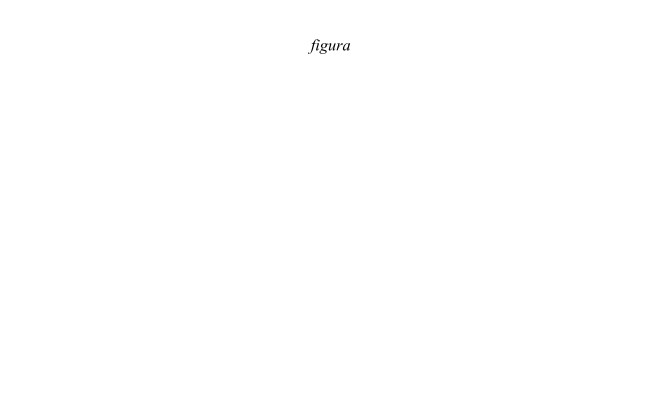
\includegraphics[width=0.95\linewidth]{figs/fig_m.jpg}		
\caption[Lorem ipsum dolor sit amet]
{\textbf{---\;Lorem ipsum dolor sit amet.}
    Lorem ipsum dolor sit amet consectetur adipiscing elit. Sed ac bibendum orci. Cras erat elit, consequat vel erat ac, tincidunt pulvinar lacus. \;\textbf{a}\;---\;Sed ac bibendum orci. Cras erat elit, consequat vel erat ac, tincidunt pulvinar lacus. Pellentesque vitae consectetur quam. Interdum et malesuada fames ac ante ipsum primis in faucibus.\;\textbf{b}\;---\;Sed ac bibendum orci. Cras erat elit, consequat vel erat ac, tincidunt pulvinar lacus. Pellentesque vitae consectetur quam. Interdum et malesuada fames ac ante ipsum primis in faucibus. \;\textbf{c}\;---\;Sed ac bibendum orci. Cras erat elit, consequat vel erat ac, tincidunt pulvinar lacus. Pellentesque vitae consectetur quam. Interdum et malesuada fames ac ante ipsum primis in faucibus.
}
\label{fig:hydro:topo} 		
\end{figure}

\subsection{Paradoxos}

\marginpar{
\tiny\raggedright\sffamily 
% todo
Falta articular a Figura. Fotos, \gls{percept-model} esquemático.
}

\par O escoamento subterrâneo translacional, por sua vez, é especulado conceitualmente por Hewlett \& Hibbert (1967) \cite{Hewlett1967}, em um artigo claramente revolucionário no campo da \gls{hydrology} \cite{McDonnell2009}. Ao mesmo tempo que criticam o \gls{paradigma} hegemônico da época (a \gls{teoria} da capacidade de infiltração), os autores organizam novos conceitos relevantes, como os termos \say{respostas rápidas e lentas} e \say{área de contribuição variável}, pavimentando o caminho para o advento do novo \gls{paradigma}. Nessa direção, os autores sugerem um mecanismo de resposta subterrânea \textit{instantânea} que ocorreria quando a \gls{fmc} do solo é superada pela infiltração da água da chuva nas zonas de fundo de vale, onde há maior influência das franjas de capilaridade. Em resumo, eles postulam que essa resposta, ainda que rápida, não seria exatamente a água da chuva, mas água que se alojou na matriz do solo \textit{antes} do evento ocorrer. Nesse processo, a espessura dos filmes de águas nas partículas do solo na \gls{unsat-zone} atingem subitamente um limite em que a rede de poros torna-se pressurizada pela gravidade. Por isso, a \textbf{água nova} da chuva (água do evento) desencadeia um pulso, uma onda de pressão, que expele a água armazenada no solo na base da encosta, uma \textbf{água velha} (água pré-evento):

\begin{adjustwidth}{100pt}{0pt}
\medskip
\small
No entanto, da parte que contribui para o escoamento, uma fração será de algumas das gotas que literalmente caíram durante a tempestade -- ou seja, um pouco de chuva nova -- e a outra fração será o que podemos chamar de \textit{fluxo translacional}, ou fluxo produzido por um processo de substituição. Esta é uma contribuição para o escoamento de água já armazenada no manto do solo antes do início da chuva. Ela será liberada em grandes quantidades apenas quando o solo estiver dentro da faixa de \gls{fmc} ou mais úmido. Acima da \gls{sat-zone}, podemos considerar esse movimento como devido ao espessamento dos filmes de água que envolvem as partículas do solo e a um pulso resultante de fluxo de água à medida que a saturação ocorre.
\footnote{Tradução livre de: 
\textit{
However, of the part contributed to direct runoff, a fraction will be some of the actual drops that fell during the storm -- that is, some new rain -- and the other fraction will be what we might call translatory flow, or flow produced by a process of displacement. This is a contribution to direct flow of water already stored in the soil mantle before rainfall began. It will be released in large quantities only when the soil is within field capacity range or wetter. Above the zone of saturation, we may regard such movement as due to thickening of the water films surrounding soil particles and a resulting pulse of water flux as the saturated zone is approached.
}} -- Hewlett \& Hibbert (1967, p. 279) \cite{Hewlett1967}.
\medskip
\end{adjustwidth}

\par Ainda que a \gls{teoria} faça sentido e cite estudos em laboratório, o texto de Hewlett \& Hibbert (1967) não oferece evidências empíricas obtidas em campo para justificar a realidade desse mecanismo. Mas isso deixou de ser uma lacuna a partir de Pinder e Jones (1969) \cite{pinder1969}, que avaliaram a separação do hidrograma de enchentes em três bacias monitoradas na Nova Escócia (entre 647,5 ha a 13,5 km², Canadá). Ao contrário dos métodos gráficos convencionais, eles inferiram a separação entre \gls{sf-runoff} e subterrâneo com marcadores químicos e um \gls{model} simples de balanço de massa\footnote{O \gls{model} desenvolvido consiste em dois compartimentos de mistura: $C_{tr}Q_{tr} =C_{dr}Q_{dr} + C_{gw}Q_{gw}$, em que: $C$ é a concentração de algum soluto conservativo; $Q$ é a vazão; $tr$ denota vazão total; $dr$ denota o escoamento direto, e; $gw$ denota o escoamento subterrâneo.}. No caso apresentando, foram monitoradas as concentrações de sódio, cálcio, bicarbonato, magnésio e sulfato antes e durante os eventos de enchentes. Os resultados indicaram uma prevalência substancial de escoamento subterrâneo durante as enchentes, com 32\% a 42\% da vazão máxima do hidrograma. Isso, porém, não eliminava a explicação alternativa de uma resposta subsuperficial da água da chuva (água nova) que dissolvera os solutos monitorados ao transitar rapidamente pelo solo. Evidências a favor da água subterrânea (água velha) tornarem-se muito mais robustas com o advento do monitoramento de isótopos de hidrogênio e oxigênio, como Deutério ($^{2}\text{H}$), Trítio ($^{3}\text{H}$) e Oxigênio-18 ($^{18}\text{O}$), marcadores ideais que fazem parte da própria molécula de água\footnote{Ao contrário de solutos comuns, a concentração de $^{18}\text{O}$ é medida pela diferença em partes por mil ($\delta^{18}\text{O}$ \textperthousand) da razão de $^{18}\text{O}/^{16}\text{O}$ de um padrão e a amostra: $\delta^{18}\text{O} = (\frac{^{18}\text{O}/^{16}\text{O} \,\text{amostra}}{^{18}\text{O}/^{16}\text{O}\,\text{padrão}} - 1) \times 1000$. O padrão costuma ser a água média dos oceanos (\texttt{SMOW} -- \textit{Sea Mean Ocean Water}). Águas desprovidas de $^{18}\text{O}$ em relação ao padrão exibem $\delta^{18}\text{O}$ negativo, e vice-versa.}. Em locais com grande variabilidade na \textbf{\gls{iso_sign}} da água precipitada, é possível se estimar o quanto dessa água nova se faz presente durante as enchentes\footnote{Obviamente, se a água da chuva for indistinguível em termos isotópicos da água no rio logo antes do evento, então é impossível extrair alguma informação relevante.}. Essa estratégia foi sugerida por Dinçer \textit{et al.} (1970) \cite{dincer1970} em um estudo nas montanhas da Tchecoslováquia que demonstrou o efeito do \textbf{\gls{term_frac}}\footnote{A principal causa da fracionamento desses isótopos na atmosfera decorre da diferença de pressão de vapor entre moléculas de água isotopicamente pesadas e leves: ${\text{H}_{2}}^{18}\text{O}$ tem uma pressão de vapor mais baixa do que  ${\text{H}_{2}}^{16}\text{O}$ e, portanto, ${\text{H}_{2}}^{16}\text{O}$ permanece preferencialmente na fase líquida tanto nos processos de evaporação quanto de condensação. Por isso, as concentrações observadas de $\delta^{18}\text{O}$ na precipitação tendem a ser incrementalmente negativas à medida que as massas de ar úmido avançam sobre os continentes \cite{sklash1976}.} nas concentrações de $^{3}\text{H}$ e $^{18}\text{O}$ em camadas de neve precipitadas e derretidas ao longo das estações. A seguir, os resultados publicados por Martinec \textit{et al.} (1974) \cite{martinec1974} notam que a água de rios nas montanhas da Suíça exibia uma concentração de $^{18}\text{O}$ com variabilidade relativamente baixa, que se aproximava da média de longo prazo das oscilações sazonais observadas na precipitação. A estratégia então assumiu contornos bem definidos com o artigo de Sklash \textit{et al.} (1976) \cite{sklash1976}, que além de organizar a lógica do método, mostra que em duas bacias monitoradas em Ontário (Canadá), a contribuição da água subterrânea na vazão máxima das enchentes foi entre 55\% (em bacias de montante) até 70\% (nas bacias de jusante, drenando uma área de 700 km$^2$). São resultados com conotações revolucionárias:

\begin{adjustwidth}{100pt}{0pt}
\medskip
\small
A descoberta mais importante é que a componente pré-evento da enchente de 16 de Maio foi grande. Por exemplo, no pico da vazão total, a componente pré-evento do arroio Big Otter em Viena foi de 70 $\pm$ 9\% do escoamento da enchente. Esses resultados substanciam as descobertas de Pinder \& Jones (1969) e Fritz \textit{et al.} (1974), embora as bacias no presente estudo sejam de uma a duas ordens de magnitude maiores em extensão de área. Esses resultados não são consistentes com os resultados simulados de Freeze (1972b), os resultados de campo de Dunne \& Black (1970a,b), e Hewlett \& Hibbert (1967), ou as implicações teóricas de Horton (1933). Os resultados são particularmente encorajadores, no entanto, à luz da grande componente subsuperficial (pré-evento) do derretimento da neve observado por Dinçer \textit{et al.} (1970).
\footnote{Tradução livre de: 
\textit{
The most important finding is that the pre-storm component of storm runoff for the 16 May storm was large. For example, at peak total discharge, the pre-storm component of Big Otter Creek at Vienna was 70 $\pm$ 9\% of storm runoff. These results substantiate the findings of Pinder \& Jones (1969) and Fritz et al. (1974), even though the basins in the present study are one to two orders of magnitude larger in areal extent.These results are not consistent with the simulated results of Freeze (1972b), the field results of Dunne \& Black (1970a,b), and Hewlett \& Hibbert (1967), or the theoretical implications of Horton (1933). The results are particularly encouraging, though, in light of the large subsurface (prestorm) component of snowmelt noted by Dinçer et al. (1970).
}} -- Sklash \textit{et al.} (1976, p. 276) \cite{sklash1976}.
\medskip
\end{adjustwidth}

\noindent Michael Sklash prosseguiu com estudos desse tipo, corroborando a existência desse processo em bacias no Canadá, na Nova Zelândia e nas Ilhas Britânicas \cite{sklash1979, sklash1986, sklash1996}. Por exemplo, o artigo de Sklash \& Farvolden (1979) \cite{sklash1979}, no Canadá, traz resultados semelhantes para uma bacia com agricultura intensiva (1 km$^2$, na Bacia Experimental Hillman Creek, Ontário) e duas bacias altamente florestadas (1,2 km$^2$ e 3,9 km$^2$, Bacia Experimental Ruisseau des Eaux Volées, Québec). Além de reportar a prevalência surpreendente da água velha nas enchentes (entre 80\% a 94\% to total escoado), os autores alimentam a \gls{teoria} das subidas rápidas da água subterrânea nos fundos de vale para explicar o fenômeno. Na Bacia Experimental de MaiMai (Nova Zelândia), Sklash \textit{et al.} (1986) \cite{sklash1986} trazem resultados que revisam drasticamente as interpretações de Mosley (1979) \cite{Mosley1979}. Citado acima, Mosley (1979) argumenta sobre a dominância nessa bacia do \gls{subsur_flow} (água nova). A prevalência inequívoca de água velha nas enchentes, obtida com os marcadores isotópicos, trouxe um certo impasse na \gls{comunidade-cientifica}, que passou desde então a propor mecanismos plausíveis \cite{buttle1994}. Nesse contexto, McDonnell (1990) \cite{mcdonnell1990} faz uma síntese dos mecanismos de resposta na bacia de MaiMai, trazendo o conceito de \textbf{ativação do escoamento subterrâneo} a partir da entrada da água da chuva na rede de macroporos das encostas, ou seja, pelo \gls{subsur_flow}. Nesse esquema, ele ressalta o papel de atalhos \textit{verticais} no perfil do solo, criado por macroporos, que fazem a água nova da chuva rapidamente se alojar nas franjas capilares da \gls{sat-zone}, criando então a ativação da carga hidráulica necessária para expulsar rapidamente a água subterrânea velha na base da encosta. Uma nova revisão, trazida por McGlynn \textit{et al.} (2002) \cite{mcglynn2002}, apresenta também o efeito relevante da \textbf{\gls{bedrock_topo}} da encosta (o embasamento de rocha relativamente impermeável). Sugere-se que as irregularidades dessa camada podem criar zonas de estagnação que armazenam a água no subsolo por tempos muito mais longos que o esperado. A eventual ativação hidráulica dessas partes mais inacessíveis expelem água velha na base da encosta. De fato, a influência das estruturas geológicas subjacentes no afloramento da água subterrânea já eram mencionadas por Huff \textit{et al.} (1982) \cite{Huff1982}, mas sem a análise da idade da água com isótopos.

\par As evidências, impasses e mecanismos plausíveis propostos para explicar a dominância da água velha nas respostas rápidas ainda aumentam em complexidade diante dos resultados da assinatura química, que tende a apresentar uma alta variabilidade. Nesse sentido, Burns \textit{et al.} (2001) \cite{burns2001quantifying} sugerem que as resposta superficiais da Bacia Experimental da Montanha Panola (Geórgia, Estados Unidos) acabam se misturando com água subterrânea na zona ripária antes de adentrar nos canais. Seibert \textit{et al.} (2003) \cite{seibert2003groundwater}, também salientam as diferentes assinaturas químicas da água da zona ripária (condições anóxicas) da água dos solos das encostas bem-drenadas (maior aeração). Essa complexidade trouxe uma certa perplexidade, expressada por Kirchner (2003) \cite{Kirchner2003} no assim chamado \textit{paradoxo duplo da hidrologia e geoquímica de bacias}\footnote{Tradução livre de \textit{douple paradox in catchment hydrology and geochemistry}.}, ou simplesmente \textbf{\gls{old_water_paradox}}. Para ele, esse paradoxo possui duas componentes que, apesar de relacionadas, são um tanto contraditórias: (1) hidrologia: a mobilização rápida de água velha -- a substituição rápida da água velha pela nova que o \gls{trans_flow} postula, e; (2) geoquímica: a variabilidade química da água velha -- o fato de que a água velha assume diferentes assinaturas químicas, a depender da velocidade de escoamento. Nesse sentido, com base nas concentrações de Cloreto\footnote{Uma estratégia análoga à feita com isótopos é possível em bacias com deposição de aerossol marinho, sendo o Cloreto um marcador inerte que pode ser analisado na água da chuva.} monitoradas em uma bacia no País de Gales, Kirchner \textit{et al.} (2000) \cite{kirchner2000} propõe uma \textbf{\gls{geo_hydro_sep}} do solo, onde os poros e fraturas exibem uma estrutura fractal de tempos de residências. Isso implicaria por que as encostas das bacias transmitem \textit{sinais hidrológicos} muito mais rápido que \textit{sinais geoquímicos}. Esse conceito torna-se mais claro por Iorgulescu \textit{et al}. (2007) \cite{Iorgulescu2007}, que reforçam a diferença entre a velocidade \textit{de onda} (celeridade) da água e a velocidade \textit{da molécula} da água -- além de material, o fluxo das enchentes é um fluxo de energia. Com o mesmo espírito, McDonnell (2014) \cite{mcdonnell2014} também desenha um novo olhar sobre os fluxos de evapotranspiração, em especial sobre a idade da água que as plantas consomem, propondo a possibilidade da \textbf{\gls{eco_hydro_sep}} do solo, o que ele denomina de \textbf{\gls{two_world}}. Evaristo \textit{et al.} (2015) \cite{Evaristo2015} trazem evidências a favor dessa \gls{hipotese}, mostrando que a separação ecológica é comum em vários biomas -- as plantas usam água do solo com uma \gls{iso_sign} distinta da água que contribui para a \gls{qv} de água subterrânea e para o escoamento fluvial.

% figure
\begin{figure}[t!] 
\centering				
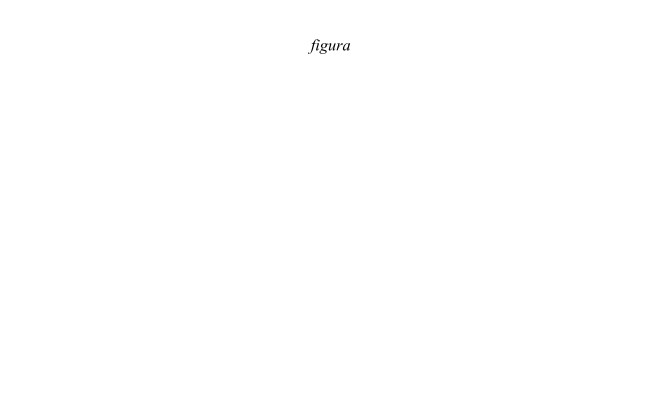
\includegraphics[width=0.95\linewidth]{figs/fig_m.jpg}		
\caption[Lorem ipsum dolor sit amet]
{\textbf{---\;Lorem ipsum dolor sit amet.}
    Lorem ipsum dolor sit amet consectetur adipiscing elit. Sed ac bibendum orci. Cras erat elit, consequat vel erat ac, tincidunt pulvinar lacus. \;\textbf{a}\;---\;Sed ac bibendum orci. Cras erat elit, consequat vel erat ac, tincidunt pulvinar lacus. Pellentesque vitae consectetur quam. Interdum et malesuada fames ac ante ipsum primis in faucibus.\;\textbf{b}\;---\;Sed ac bibendum orci. Cras erat elit, consequat vel erat ac, tincidunt pulvinar lacus. Pellentesque vitae consectetur quam. Interdum et malesuada fames ac ante ipsum primis in faucibus. \;\textbf{c}\;---\;Sed ac bibendum orci. Cras erat elit, consequat vel erat ac, tincidunt pulvinar lacus. Pellentesque vitae consectetur quam. Interdum et malesuada fames ac ante ipsum primis in faucibus.
}
\label{fig:hydro:paradox} 		
\end{figure}

\section{Escala} \label{sec:hydro:scale}

\par Acompanhando a revolução científica causada pelas evidências empíricas sobre os mecanismos de escoamento nas encostas, a década de 1960 também foi marcada pelo advento dos primeiros modelos hidrológicos simulados em computadores digitais. Isso ocorreu em grande medida por uma confluência de fatores, como o contexto intelectual da Teoria Geral dos Sistemas de von Bertalanffy e das práticas da \gls{sys-dyn} de Jay Forrester, que seguiam a emergência dos computadores digitais do tipo \textit{mainframe}. Keith Beven relata que em 1971 ele havia contado mais de uma centena de modelos hidrológicos na literatura, que eram basicamente versões do \gls{model} da Universidade de Stanford, o \textit{Stanford Watershed Model IV} (\texttt{SWM}) \cite{Beven2019a}. O \gls{model} fora desenvolvido a partir de 1959 como tese de doutorado de Norman Crawford, orientado por Ray Linsley, e depois acabou dando origem a um programa denominado \textit{Hydrologic Simulation Program, Fortran} (\texttt{HSPF}), desenvolvido para e com o suporte da U.S. Environmental Protection Agency (\texttt{USEPA}) \cite{Burges2004a}. Esse \gls{model}, tido como pioneiro, exemplifica claramente a influência da ontologia oferecida pela \gls{sys-dyn}: uma rede de reservatórios conectados por fluxos que é resolvida numericamente. No caso, o SWM é apenas um pouco mais intrincado que o \gls{model} minimalista apresentado no capítulo anterior, com quatro reservatórios (dossel, \gls{unsat-zone}, \gls{sat-zone} e canais de drenagem) e três mecanismos de resposta (incluindo uma resposta subsuperficial além do \gls{sf-runoff} e subterrâneo). O \gls{model}, porém, não representa o armazenamento de água na superfície, tampouco diferencia aspectos topográficos de maneira que o \gls{sf-runoff} possa ser separado em excesso de infiltração ou excesso de saturação. Mas isso não é exatamente um problema na \gls{sys-dyn}, basta acrescentar um novo compartimento e ir conectando os fluxos. A flexibilidade provida pela \gls{sys-dyn}, nesse sentido, a introduziu como um \gls{paradigma} conceitual e procedural na modelagem hidrológica, resultando tanto na profusão de modelos a partir desse período, quanto ao entendimento teórico da importância da \textbf{escala} em todo o processo de modelagem.

\subsection{Modelos baseados em dados}

\par Antes do advento das simulações hidrológicas, porém, a abordagem para se obter hidrogramas de enchentes a partir de dados de chuvas baseava-se primordialmente no conceito de \textbf{\gls{unit_hydro}} da bacia, introduzido por Sherman (1932) \cite{Sherman1932a}. Esse conceito se fundamenta na tese de que a \gls{hydro-response} de uma bacia resume-se a um processo linear de propagação cinemática na rede de canais a partir de um pulso de chuva, que pode ser reduzido a um pulso unitário. Segundo o \textbf{princípio da sobreposição}, pulsos mais complexos de chuva podem ser integrados no tempo (método da convolução). Nesse caso, o parâmetro fundamental de uma bacia consiste no seu \textbf{\gls{time_conc}}, que é relativamente maior em bacias alongadas do que em bacias arrendondadas, mesmo que possuam exatamente a mesma área. A visão sistêmica permitiu que esse processo fosse representado como uma rede de reservatórios organizados em série, uma \say{cascata}, fato que resulta na parametrização de uma distribuição Gama, ou [todo:gls >> \textbf{modelo de Kalinin-Miyukov-Nash} >> nash-model]:
\begin{linenomath*}
\begin{equation}
\label{eq:kalinin}
Q(t) = \frac{\nu}{k\; \Gamma(n)} e^{-t/k} (t/k )^{n-1}
\end{equation}
\end{linenomath*}
\noindent Em que $n$ pode ser interpretado como o número efetivo de reservatórios, e; $k$ pode ser interpretado como o tempo de residência médio dos reservatórios. Ao que consta, essa parametrização foi obtida de forma independente primeiro por Kalinin \& Miyukov (1957) \cite{Kalinin1957a}, na União Soviética, e depois por Nash (1958), na Inglaterra \cite{Nash1958a}. A partir disso, surgiu a noção de que a resposta da bacia é análoga a uma \textit{função} ou \textit{filtro} que atua sobre o sinal da chuva (ou outros sinais de entrada). Essa abordagem de se obter hidrogramas, que é um \gls{paradigma} de modelagem, evoluiu a partir disso no que Todini \cite{Todini2007a} denomina de \textbf{\gls{models_data}}, em contraste com os \textbf{\gls{models_process}}. Os \gls{models_data} são hoje um conjunto de técnicas que inclui, por exemplo, redes neurais artificiais. Essa abordagem é visivelmente contaminada pelo \gls{bias-fluvial}, afinal, não é possível \textit{explicar} exatamente onde e como que o escoamento foi gerado a partir de uma \gls{teoria} verdadeiramente hidrológica -- a bacia é tida como uma caixa-preta. Nessa linha, Todini argumenta que essa família de modelos buscou maximizar a \textbf{\gls{pred_cap}} em detrimento da \textbf{\gls{explan_cap}}, ou seja, de produzir resultados que tenham \say{significado físico}. Uma tentativa de se re-estabelecer a \gls{explan_cap} de \gls{models_data} é a abordagem de modelagem denominada de \textit{Data Based Mechanistic} (\texttt{DBM}), esquematizada por Young (2002) \cite{Young2002a}. Essa técnica resulta não somente em predições de vazão, mas também identifica estruturas e \gls{parameters} internos que possuem \gls{explan_cap}. Diante disso, Todini argumenta:
\begin{adjustwidth}{100pt}{0pt}
\medskip
\small
Embora a abordagem de modelagem \texttt{DBM} reconheça a importância da coerência física da estrutura do \gls{model} identificado, ela a deriva das observações, desconsiderando \textit{de fato} os resultados de pelo menos 50 anos de esforços de pesquisa voltados para especificar os mecanismos hidrológicos físicos que geram as enchentes. Isso contrasta com o princípio de Bayes, que combinaria as observações com todo o conhecimento \textit{a priori} possível sobre os processos hidrológicos e possivelmente sobre os valores dos \gls{parameters} para obter previsões \textit{a posteriori} menos incertas.
\footnote{Tradução livre de: 
\textit{
Although the DBM modelling approach recognises the importance of the  physical coherence of the identified model structure, it derives it from the observations, thus disregarding de facto the results of at least 50 years of research efforts aimed at specifying the physical hydrological mechanisms that generate floods. This contrasts with the Bayes principle which would combine the observations with all possible a priori knowledge on the hydrological processes and possibly on the parameter values to obtain less uncertain a posteriori forecasts.
}} -- Todini (2007, p. 471) \cite{Todini2007a}.
\medskip
\end{adjustwidth}
\noindent Como salientado no Capítulo \ref{chap:episteme}, \textit{modelos são veículos simbólicos de teorias}. Nesse sentido, \gls{models_data} são, em sua essência, \textbf{modelos estatísticos}: eles estabelecem uma \gls{teoria} sobre os dados \textit{em si}, sobre as suas relações internas. Como mencionado no Capítulo \ref{chap:systems}, tais modelos tendem a ser \textit{sobre-ajustados aos dados}, fato que permite boas interpolações mas torna as extrapolações problemáticas, não contribuindo no processo de aprendizado que a \gls{sys-dyn} oferece. Os modelos baseados em \textit{processos}, por outro lado, instanciam uma representação sobre um \textit{sistema-alvo} que existe em uma realidade objetiva \textit{para além} dos dados -- a bacia hidrográfica. Por isso, um \gls{model} verdadeiramente hidrológico, baseado em processos, é capaz de simular o comportamento de uma bacia \textit{mesmo sem nenhuma observação empírica disponível} (um cenário sintético, por exemplo), pois a modelagem é um processo de \textbf{inferência dedutiva}. O papel das evidências empíricas, nesse sentido, é de rejeitar ou corroborar a \gls{teoria} veiculada pelo \gls{model}.

\subsection{Incomensurabilidade}

\par Apesar da atratividade em termos da \gls{explan_cap}, os \gls{models_process}, viabilizados pela \gls{sys-dyn}, também passaram a demonstrar as suas limitações, especialmente diante das evidências supostamente associadas aos \gls{parameters}. Mesmo representando mecanismos de \gls{hydro-response} conhecidos, a natureza altamente \textit{agregada} dos compartimentos instanciados deixou cada vez mais nítido que definir os \gls{parameters} de um \gls{model} hidrológico para se obter bons resultados não era uma prática trivial, exigindo um longo processo de tentativa e erro, marcado por muitas nuances\footnote{Segundo Keith Beven, nos primórdios da modelagem de chuva-vazão, havia uma história de que a única pessoa que conseguia realmente calibrar o Modelo de Stanford, com todos os seus \gls{parameters}, era Norman Crawford, que escreveu a versão original do \gls{model} como parte de sua tese de doutorado (Beven 2012, p. 233 \cite{Beven2012}).}. Para piorar, os valores dos \gls{parameters} que produziam resultados aderentes às observações empíricas raramente coincidiam com valores medidos em campo. Por exemplo, Amorocho \& Hart (1964) [todo:cite] chamam a atenção para resultados irreais obtidos internamente nesse tipo de \gls{model}, devido a \textbf{\gls{comp-eff}} no balanço de massa imposto aos compartimentos. Por essa razões, Todini sugere que calibrar modelos hidrológicos com métodos de otimização sem maiores preocupações com a coerência física dos \gls{parameters} acaba, na prática, transformando um \gls{model} baseado em processos em um \gls{model} baseado em dados, pois o foco tende a ser ajustar \gls{input-data} (chuva) e saída (vazão), e não explicar fenômenos em uma realidade objetiva \cite{Todini2007a}. Essa limitação deriva de dois problemas inexoráveis e indissociáveis da modelagem hidrológica: (1) o \textbf{\gls{problem-equifinal}} e, (2) o \textbf{\gls{scale_problem}}. 

\par O \gls{problem-equifinal} foi explorado no Capítulo \ref{chap:episteme} (Seção \ref{sec:epis:under}), sendo uma versão mais branda do \gls{problem-subdet} de teorias que postulam entidades inobserváveis. O termo \say{equifinalidade} foi introduzido por von Bertalanffy na Teoria Geral dos Sistemas (Capítulo \ref{chap:systems}, Seção \ref{sec:sys:systems}), transmitindo a noção de que \gls{sys-open} diferentes podem convergir para estruturas similares. Na modelagem, está associado ao fato de que sistemas com estruturas ou mesmo \gls{parameters} distintos podem exibir \textit{comportamentos} similares, como no caso das respostas lentas ilustradas no protótipo de \gls{model} da Seção \ref{sec:systems:model}. Assim, o \gls{proc-calib} de um \gls{model} com informações parciais sobre seus processos (apenas a vazão observada, por exemplo), \textbf{não} garante que os outros processos internos estejam adequadamente representados em termos empíricos -- por isso a discrepância entre \gls{parameters} observados e ajustados. Mas mesmo que \textit{existam} informações completas, o \gls{scale_problem} implica que as diferenças entre a escala que o \gls{model} representa e a escala das observações são \textit{incomensuráveis}, ou incompatíveis, introduzindo o \gls{error-commensu} $\varepsilon_{\Delta}$ nos resultados do \gls{model} (ver a Equação \eqref{eq:total-error}, a \gls{eq-total-error}). Cabe ressaltar que a questão da \gls{scale-similarity} foi um problema foi prontamente reconhecido no campo dos \gls{scale-models} reduzida, mas só foi apreciado a partir da década de 1980 na modelagem hidrológica.

\subsection{Modelos fisicamente embasados}

\par Diante das dificuldades de compatibilizar observações de campo com os ajustes dos sistemas modelados e a crescente capacidade computacional disponível pelos \textit{mainframes}, Freeze \& Harlan (1969) inauguraram uma nova visão sobre a modelagem hidrológica, originando o que eles denominaram de \textbf{\gls{models-phys}}. Essa forma de modelagem, assim como na \gls{sys-dyn}, é baseada da descrição de processos. A diferença, no entanto, é que os processos descritos por esses modelos são derivados \textit{diretamente} de leis postuladas pela Física: a conservação de massa, momento e energia. O artigo de Freeze \& Harlan estabeleceu um \say{projeto} de \gls{model} fisicamente embasado que difere fundamentalmente da \gls{sys-dyn} em seus aspectos ontológicos. Ao contrário do \gls{paradigma} sistêmico, que se fundamenta em compartimentos agregados conectados por fluxos e retroações, no \gls{paradigma} físico existem apenas \textbf{campos vetoriais} de velocidade que atuam continuamente, distribuídos no domínio do espaço tridimensional $\mathbb{R}^3$ e modulados pelas condições iniciais e de contorno. Com isso, os autores tinham como objetivo explícito oferecer uma alternativa superior aos modelos sistêmicos:
\begin{adjustwidth}{100pt}{0pt}
\medskip
\small
Com os modelos de sistemas hidrológicos, é possível simular hidrogramas do escoamento fluvial com um alto grau de precisão para uma variedade de condições hidrológicas e geográficas. O Stanford Watershed Model IV (Crawford e Linsley) é o \gls{model} mais conhecido e bem-sucedido desse tipo. Se o \gls{model} que defendemos for promissor para o futuro, ele deve ser capaz de competir com a abordagem de sistemas em termos de resultados práticos e utilidade. Pode-se então argumentar a favor de sua superioridade com base no fato de que uma melhor compreensão dos processos internos e seus efeitos no \gls{system} hidrológico como um todo é desejável e pode ser benéfica para a solução de problemas práticos.
\footnote{Tradução livre de: 
\textit{
With hydrologic systems models, it is possible to simulate streamflow hydrographs with a high degree of accuracy for a variety of hydrologic and geographic conditions. The Stanford Watershed Model IV (Crawford and Linsley), is the best-known and most successful model of this type. If the model we espouse is to offer promise for the future, it must be able to compete with the systems approach in terms of practical results and utility. A case could then be made for its superiority on the basis that a better understanding of the internal processes and their effects on the overall hydrologic system is desirable and could be beneficial to the solution of practical problems.
}} -- Freeze \& Harlan (1969, p. 242) \cite{Freeze1969a}.
\medskip
\end{adjustwidth}
\noindent Ou seja, os autores apostavam que a saída para evitar os problemas já aparentes no \gls{proc-calib} de modelos da \gls{sys-dyn} era aplicar as leis da Física (Mecânica de Fluidos) diretamente para descrever o \gls{hydro_cicle} nas bacias -- afinal, não era necessário reinventar a roda. O único entrave talvez fosse a capacidade computacional disponível, ainda que por outro lado não seria necessário calibrar os modelos por qualquer método de busca intensivo, já que os \gls{parameters} \textit{verdadeiramente} físicos poderiam ser definidos \textit{a priori}, como a rugosidade de canais, ou a condutividade hidráulica. Outra vantagem prometida era a capacidade de integração contínua entre as partes dos \gls{system}, como o \gls{sf-runoff} e escoamento subterrâneo. Eles apontam que, apesar de certos processos do \gls{hydro_cicle} na época ainda carecerem de estudos fisicamente embasados (como os processos de evaporação), o escoamento unidimensional em canais e tridimensional em meio poroso já estavam bem estabelecidos pelas equações de St. Venant e Darcy-Richards, respectivamente. Variações para diferentes condições de contorno ou \gls{neglig-premis} poderiam ser desenvolvidas e soluções obtidas em novos estudos teóricos.

\par Um bom exemplo da abordagem fisicamente-embasada (e suas problemáticas) é a modelagem do escoamento em meio poroso, a água no solo. Nesse caso, a lógica emerge a partir da \textbf{\gls{darcy-law}}. Essa lei foi obtida experimentalmente por Henry Darcy (1803-1858) com uma tubulação preenchida com areia, onde ele observou que a vazão de água na tubulação $Q \; [\text{L}^{3}\text{T}^{-1}]$ é diretamente proporcional à área da seção da tubulação $A \; [\text{L}^{2}]$ e à diferença de potencial hidrostático entre a entrada e a saída $\Delta z \; [\text{L}]$ \cite{Simmons2008a}. Ao mesmo tempo, a vazão é inversamente proporcional ao comprimento da tubulação $l \; [\text{L}]$. Para transformar essas relações em uma equação com consistência dimensional, é introduzida a \textbf{condutividade hidráulica} $K \; [\text{L}\,\text{T}^{-1}]$ \footnote{Para qualquer fluido e qualquer meio poroso $K$ se define por: $K = \frac{c}{\mu}$, em que $c \; [\text{M}\,\text{T}^{-2}]\;$ é a permeabilidade do meio poroso, e; $\mu \; [\text{M}\,\text{L}^{-1}\,\text{T}^{-1}]$ é a viscosidade do fluido.}:
\begin{linenomath*}
\begin{equation}
\label{eq:darcy}
Q  = K \frac{A}{l}\Delta z 
\end{equation}
\end{linenomath*}
\noindent Essa é uma análise na \textbf{\gls{glob-scale}}, ou seja, avaliando o comportamento \textit{agregado} do \gls{system} da tubulação. Mas então é realizado um movimento analítico crucial para se migar para a \textbf{\gls{loc-scale}}. Isso é feito ao se \textit{assumir} que é possível representar \textit{elementos infinitesimais} do solo, o que leva à definição do gradiente de potencial hidrostático $\nabla \Phi \; [\text{L}\text{L}^{-1}]$:
\begin{linenomath*}
\begin{equation}
\label{eq:darcy-2}
\nabla \Phi = \frac{\Delta z}{l} 
\end{equation}
\end{linenomath*}
\noindent Portanto, da Equação \eqref{eq:darcy} segue que:
\begin{linenomath*}
\begin{equation}
\label{eq:darcy-3}
Q/A = K \nabla \Phi \quad \Rightarrow \quad u = K \nabla \Phi
\end{equation}
\end{linenomath*}
\noindent Em que $u \; [\text{M}\,\text{T}^{-2}]$ é a \textbf{velocidade darciana}\footnote{A \textbf{velocidade real} do fluido é maior, uma vez que o fluido precisa escoar por uma seção relativamente menor, onde existem poros que sejam conectados.} do fluido. Para um domínio espacial tridimensional $\mathbb{R}^3=\{x, y, z \}$:
\begin{linenomath*}
\begin{equation}
\label{eq:darcy-4}
u_x = - K\frac{\partial \Phi}{\partial x} \quad 
u_y = - K\frac{\partial \Phi}{\partial y} \quad 
u_z = - K\frac{\partial \Phi}{\partial z}
\end{equation}
\end{linenomath*}
\noindent Que faz a \gls{darcy-law} assumir a seguinte notação diferencial e vetorial\footnote{O sinal negativo denota que o sentido da velocidade é o contrário do gradiente de potencial hidrostático.}:
\begin{linenomath*}
\begin{equation}
\label{eq:darcy-5}
\textbf{u} = - K \nabla \Phi
\end{equation}
\end{linenomath*}

\par A manobra para \textit{colapsar} a \gls{glob-scale} em uma \gls{loc-scale} de elementos infinitesimais é uma típica \textbf{\gls{idealization} galileana}, quando se deduz matematicamente uma representação em uma \textit{condição limite} partindo-se da representação de uma \textit{condição observada}  (ver Seção \ref{sec:sys:represent}). Galileu usou o plano inclinado para então idealizar a condição limite do ângulo vertical para objetos em queda-livre. No caso do escoamento em meio poroso, a \gls{darcy-law} para uma tubulação com areia assume a forma da Equação \eqref{eq:darcy-5} no limite de elementos infinitesimais de solo. A formulação completa para descrever o movimento da água no solo, incluindo fluxos na \gls{unsat-zone}, é descrita pela Equação de Richards (ou Darcy-Richards). Richards (1931) \cite{Richards1931a}, acoplou a Equação de Darcy com o balanço de massa na \gls{loc-scale} (nos supostos elementos infinitesimais) produzindo um \gls{system} de equações diferenciais parciais que precisam ser resolvidas no tempo e no espaço tridimensional\footnote{A Equação de Richards pode assumir diferentes notações, mas em geral ela se estabelece com a expansão do potencial hidrostático para incluir, além do potencial gravitacional $\Delta z$ também o potencial capilar da água, de forma que: $\Phi = \Delta z + \psi$. Com isso, condutividade hidráulica do fluido passa a ser variável em condições saturadas, exibindo inclusive efeitos de histerese.}. 

\par A proposta de modelagem inovadora feita por Freeze \& Harlan (1969) foi explicitamente denominada de \say{projeto}, pois não estava prontamente operacional. Mas ela já apontava as direções para novas pesquisas nas frentes teóricas e aplicadas para que um modelo completamente integrado eventualmente fosse concretizado para além das equações. Esse processo foi, em parte, liderado pelo próprio Allan Freeze, em uma série de artigos que ele apresenta os resultados de diversas simulações experimentais no âmbito do escoamento da água subterrânea \cite{Freeze1974a}. Em uma típica demonstração de modelagem exploratória, Freeze inicia esse movimento organizando os detalhes matemáticos teóricos (as equações diferenciais) e numéricos (os métodos de solução) para simular o escoamento transiente em meio poroso não-saturado no domínio tridimensional de uma encosta idealizada \cite{Freeze1971a}. O resultado obtido por Freeze consiste em uma solução pelo [todo:gls >> \textbf{método de diferenças finitas} >> finite-diff-method], com uma [todo:gls >> \textbf{malha computacional} >> comp-grid] regular que pode ser aplicada para qualquer geometria superficial de encosta e padrão subterrâneo geológico (por exemplo, soleiras impermeáveis e diferentes horizontes de solo). Alternativamente, Beven (1977) \cite{Beven1977a} demonstrou que também é possível implementar soluções numéricas pelo [todo:gls >> \textbf{método de elementos finitos} >> finite-elem-method], com a aplicação de uma a malha computacional \textit{irregular}. Com vistas de plano e perfil das variáveis simuladas, os experimentos virtuais com modelos desse tipo mostram detalhadamente o comportamento da água subterrânea diante de padrões espaciais de chuva e retirada de água por poços ou canais. Em avanços subsequentes, Freeze busca dialogar com as evidências empíricas sobre as os novos mecanismos de escoamento que estavam sendo reportados pela comunidade científica no final dos anos 1960, frisando que o modelo fisicamente embasado desenvolvido produzia tais fenômenos naturalmente, a depender apenas das condições de contorno, isto é, a geometria da encosta \cite{Freeze1972a, Freeze1972b}. Nessa linha, a teoria física indicaria que o escoamento subsuperficial seria dominante nas encostas convergentes convexas (vale encaixado) enquanto que o excesso de saturação dominaria nas encostas convergentes côncavas (vale em anfiteatro). 

\subsection{Promessas quebradas}

\par O projeto vislumbrado por Freeze \& Harlan (1969), assim, se concretizou em diversos modelos mais outros menos integrados com o ciclo hidrológico, incluindo modelos como \texttt{HEC-RAS} (focado no escoamento superficial) e \texttt{MODFLOW} (focado em escoamento subterrâneo) \cite{Simmons2020a}. Entre os modelos pioneiros e completamente integrados, destaca-se o modelo Système Hydrologique Européen (SHE) [todo:acr], que foi desenvolvido a partir de 1976 por uma colaboração entre o Danish Hydraulic Institute, o Brititsh Hydrology Institute e a empresa de consultoria francesa SOGREAH. Após dez anos de desenvolvimentos, resultados operacionais passaram a ser divulgados e a estrutura do modelo foi publicada em uma série de artigos em 1986 \cite{Abbott1986a, Abbott1986b}. Segundo os seus autores, o modelo foi explicitamente inspirado no projeto de Freeze \& Harlan (1969), ainda que tenham implementado uma versão simplificada do escoamento na zona vadosa, com uma formulação unidimensional da Equação de Darcy-Richards. Apesar de todo o esforço alocado e a complexidade computacional em comparação aos modelos baseados na Dinâmica de Sistemas, os autores do modelo \texttt{SHE} prontamente reconhecem as suas limitações, em especial o problema da escala:
\begin{adjustwidth}{100pt}{0pt}
\medskip
\small
Em princípio, como os valores dos parâmetros são baseados em medições físicas, modelos como o \texttt{SHE} não deveriam exigir calibração. Na prática, entretanto, problemas como a representação inadequada dos processos hidrológicos e a possível diferença de escala entre a medição e o elemento de malha do modelo significam que alguma calibração provavelmente continuará sendo necessária. No contexto do \texttt{SHE}, isso é feito melhorando-se seletivamente as estimativas iniciais dos parâmetros por uma comparação entre variáveis hidrológicas observadas e simuladas, como vazão ou níveis do lençol freático. Atualmente, isso é realizado por tentativa e erro.
\footnote{Tradução livre de: 
\textit{
In principle, because the parameter values are based on physical measurements, models such as the SHE should not require calibration. In practice, though, problems such as inadequate representation of the hydrological processes and the possible difference in scale between the measurement and the model grid square mean that some calibration is likely to continue to be required. In a SHE context this is regarded as a selective improvement of initial parameter estimates, by a comparison between observed and simulated hydrological variables, e.g. stream discharges or phreatic surface levels. At present this is carried out on a trial and error basis. 
}} -- Abbott \textit{et al.} (1986, p. 53) \cite{Abbott1986a}.
\medskip
\end{adjustwidth}
\noindent Esse fato claramente quebra a promessa feita por Freeze \& Harlan (1969), de que um modelo fisicamente embasado estaria livre de tais nuances, com a definição de parâmetros feitas \textit{a priori}, sem a necessidade de ajustes manuais ou automatizados \textit{a posteriori}. 

\par As limitações práticas do modelo \texttt{SHE} abriram uma brecha para a instalação de uma crise no âmbito da modelagem hidrológica, fornecendo insumos para uma discussão teórica e filosófica sobre os problemas de escala e de incertezas nos anos 1990 e 2000. Essa crise escancara-se no ensaio crítico feito por Beven (1989) \cite{Beven1989a}, que organiza sistematicamente os problemas dos modelos fisicamente embasados. Nesse momento, Beven aponta que, na prática, a modelagem fisicamente embasada aplica uma [todo:gls >> \textbf{premissa de escalabilidade} >> scale-prem], que é tão idealizadora como as demais simplificações vistas na Dinâmica de Sistemas, com a vantagem da últimoa ser mais intuitiva. Por exemplo, Beven cita a aplicação do modelo \texttt{SHE} em uma bacia na Inglaterra que instanciou elementos de malha computacional com 250 metros de comprimento, como se a física dos campos de velocidade fosse aplicável para essa escala. As variáveis simuladas em um elemento de malha com centenas de metros de comprimento claramente não são comensuráveis com evidências empíricas pontuais. Além disso, mesmo com elementos de malha relativamente pequenos (na escala de centímetros), os modelos não sub-representam os processos que sabidamente ocorrem \textit{abaixo} dessa escala. Ao contrário do escoamento livre em canais ou em aquíferos extensos e homogêneos, que são bem representados por campos de velocidade, as evidências empíricas sobre a \gls{macropor} em encostas com solos estruturados trazem incompatibilidades fundamentais com a ontologia dos modelos fisicamente embasados \cite{Beven2013a, Beven2019a}. Como foi ressaltado por Hursh \& Fletcher (1942), citados acimas, \say{Um único túnel de minhoca pode ser muito mais importante na drenagem de um bloco de solo maciço do que toda a área da seção transversal do espaço poroso}. Ao instanciar campos de velocidade contínuos, a Equação de Darcy-Richards simplesmente não captura a complexidade local da estrutura de macroporos do solo (ou, equivalentemente, fissuras em um aquífero fraturado). Do ponto de vista científico, Kirchner 2006 \cite{Kirchner2006a} lembra que equações diferenciais elegantes não garantes bons resultados por bons motivos -- esse é um papel reservado para as evidências empíricas e testes de hipótese.

\par Com o advento das fortes críticas e discussões, a defesa dos modelos fisicamente embasados assumiu um tom pragmático, com um discurso muito mais brando em relação ao articulado por Freeze \& Harlan (1969). Nessa linha, Woolhiser (1996) \cite{Woolhiser1996a} sugere que o desenvolvimento de modelos que representem realisticamente os processos hidrológicos diretamente da teoria física talvez tenha sido uma grande ilusão da comunidade científica, análoga à busca do \say{El Dorado}. Por outro lado, Simmons \textit{et al.} (2020) \cite{Simmons2020a}, alegam que o espírito central do projeto de Freeze \& Harlan era promover o \textit{acoplamento} entre os diversos compartimentos do ciclo hidrológico, como a atmosfera, o solo, subsolo e os rios -- e não se obter uma descrição supostamente verdadeira da realidade. Como a maior parte das críticas orbitou em torno da representação de campos contínuos (a ontologia) e suas consequências filosóficas, a essência do projeto continua viva e produzindo importantes \textit{insights} ao integrar em uma plataforma de modelagem diversas ciências, como hidrologia, climatologia e ecologia. Por essa razão, eles enfatizam que o termo \say{fisicamente embasado} induz a uma interpretação falsa dos propósitos finais, sendo \say{modelos integrados} uma denominação mais apropriada. Um fato inegável de cunho pragmático que contribui nessa direção, trazido por Fatichi \textit{et al.} (2016) \cite{Fatichi2016a}, é que problemas complexos geralmente precisam de soluções complexas. Ou seja, diversas aplicações práticas necessitam de \textit{modelos distribuídos}, que representem com detalhes suficientes os processos hidrológicos no espaço bi ou tridimensional para auxiliar na tomada de decisões envolvendo a gestão de recursos hídricos, como mapeamento de inundações e mudanças de uso do solo. Além disso, Clark \textit{et al.} (2017) \cite{Clark2017a} alegam que os problemas filosóficos de escala e incerteza, ainda que intrínsecos, estão cada vez mais assimilados por modelos distribuídos, em especial com técnicas de \textbf{regionalização} entre escalas, com parametrizações aninhadas que podem ir desde o elemento de malha mais fino (escala local), passando por escalas intermediárias, indo até a escala global do domínio da modelagem.
 
\section{Similaridade} \label{sec:hydro:sim}

\cite{Sivapalan1987a}

Equação do Wood! \cite{Wood1988a} -- REA

\par Lorem ipsum dolor sit amet consectetur adipiscing elit. Sed ac bibendum orci. Cras erat elit, consequat vel erat ac, tincidunt pulvinar lacus. Pellentesque vitae consectetur quam. Interdum et malesuada fames ac ante ipsum primis in faucibus. The typesetting markup language is specially suitable for documents that include . Given a set of numbers, there are elementary methods to compute its, which is abbreviated. Lorem ipsum dolor sit amet consectetur adipiscing elit. Sed ac bibendum orci. Cras erat elit, consequat vel erat ac, tincidunt pulvinar lacus. Pellentesque vitae consectetur quam. Interdum et malesuada fames ac ante ipsum primis in faucibus. The typesetting markup language is specially suitable for documents that include . Given a set of numbers, there are elementary methods to compute its, which is abbreviated. This process is similar to that used for the. 

\section{TOPMODEL} \label{sec:hydro:topmodel}

\par Lorem ipsum dolor sit amet consectetur adipiscing elit. Sed ac bibendum orci. Cras erat elit, consequat vel erat ac, tincidunt pulvinar lacus. Pellentesque vitae consectetur quam. Interdum et malesuada fames ac ante ipsum primis in faucibus. The typesetting markup language is specially suitable for documents that include . Given a set of numbers, there are elementary methods to compute its, which is abbreviated. Lorem ipsum dolor sit amet consectetur adipiscing elit. Sed ac bibendum orci. Cras erat elit, consequat vel erat ac, tincidunt pulvinar lacus. Pellentesque vitae consectetur quam. Interdum et malesuada fames ac ante ipsum primis in faucibus. The typesetting markup language is specially suitable for documents that include . Given a set of numbers, there are elementary methods to compute its, which is abbreviated. This process is similar to that used for the. 

% figure
\begin{figure}[t!] 
\centering				
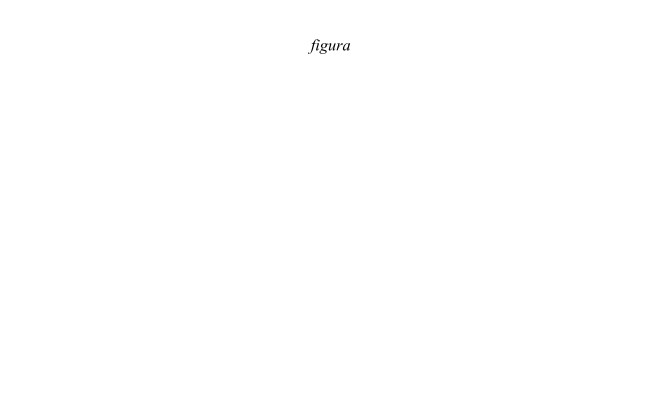
\includegraphics[width=0.95\linewidth]{figs/fig_m.jpg}		
\caption[Lorem ipsum dolor sit amet]
{\textbf{---\;Lorem ipsum dolor sit amet.}
    Lorem ipsum dolor sit amet consectetur adipiscing elit. Sed ac bibendum orci. Cras erat elit, consequat vel erat ac, tincidunt pulvinar lacus. \;\textbf{a}\;---\;Sed ac bibendum orci. Cras erat elit, consequat vel erat ac, tincidunt pulvinar lacus. Pellentesque vitae consectetur quam. Interdum et malesuada fames ac ante ipsum primis in faucibus.\;\textbf{b}\;---\;Sed ac bibendum orci. Cras erat elit, consequat vel erat ac, tincidunt pulvinar lacus. Pellentesque vitae consectetur quam. Interdum et malesuada fames ac ante ipsum primis in faucibus. \;\textbf{c}\;---\;Sed ac bibendum orci. Cras erat elit, consequat vel erat ac, tincidunt pulvinar lacus. Pellentesque vitae consectetur quam. Interdum et malesuada fames ac ante ipsum primis in faucibus.\;\textbf{d}\;---\;Sed ac bibendum orci. Cras erat elit, consequat vel erat ac, tincidunt pulvinar lacus. Pellentesque vitae consectetur quam. Interdum et malesuada fames ac ante ipsum primis in faucibus.
}
\label{fig:hydro:1} 		
\end{figure}

\section{Conectividade}

\par Lorem ipsum dolor sit amet consectetur adipiscing elit. Sed ac bibendum orci. Cras erat elit, consequat vel erat ac, tincidunt pulvinar lacus. Pellentesque vitae consectetur quam. Interdum et malesuada fames ac ante ipsum primis in faucibus. The typesetting markup language is specially suitable for documents that include . Given a set of numbers, there are elementary methods to compute its, which is abbreviated. Lorem ipsum dolor sit amet consectetur adipiscing elit. Sed ac bibendum orci. Cras erat elit, consequat vel erat ac, tincidunt pulvinar lacus. Pellentesque vitae consectetur quam. Interdum et malesuada fames ac ante ipsum primis in faucibus. The typesetting markup language is specially suitable for documents that include . Given a set of numbers, there are elementary methods to compute its, which is abbreviated. This process is similar to that used for the. 

% figure
\begin{figure}[t!] 
\centering				
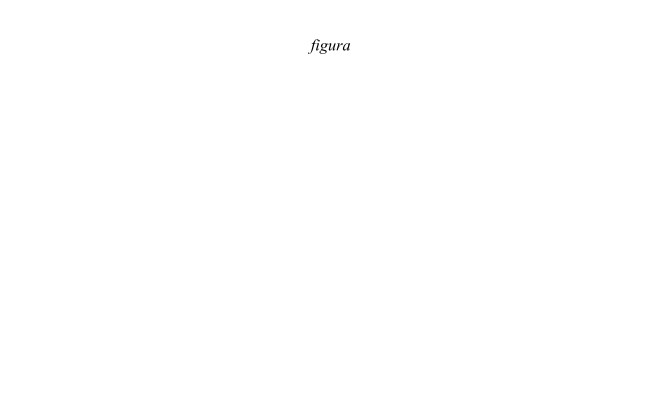
\includegraphics[width=0.95\linewidth]{figs/fig_m.jpg}		
\caption[Lorem ipsum dolor sit amet]
{\textbf{---\;Lorem ipsum dolor sit amet.}
    Lorem ipsum dolor sit amet consectetur adipiscing elit. Sed ac bibendum orci. Cras erat elit, consequat vel erat ac, tincidunt pulvinar lacus. \;\textbf{a}\;---\;Sed ac bibendum orci. Cras erat elit, consequat vel erat ac, tincidunt pulvinar lacus. Pellentesque vitae consectetur quam. Interdum et malesuada fames ac ante ipsum primis in faucibus.\;\textbf{b}\;---\;Sed ac bibendum orci. Cras erat elit, consequat vel erat ac, tincidunt pulvinar lacus. Pellentesque vitae consectetur quam. Interdum et malesuada fames ac ante ipsum primis in faucibus. \;\textbf{c}\;---\;Sed ac bibendum orci. Cras erat elit, consequat vel erat ac, tincidunt pulvinar lacus. Pellentesque vitae consectetur quam. Interdum et malesuada fames ac ante ipsum primis in faucibus.\;\textbf{d}\;---\;Sed ac bibendum orci. Cras erat elit, consequat vel erat ac, tincidunt pulvinar lacus. Pellentesque vitae consectetur quam. Interdum et malesuada fames ac ante ipsum primis in faucibus.
}
\label{fig:hydro:2} 		
\end{figure}

\clearpage

\section{Resumo do capítulo} \label{sec:hydro:summary}

\par Lorem ipsum dolor sit amet consectetur adipiscing elit. Sed ac bibendum orci. Cras erat elit, consequat vel erat ac, tincidunt pulvinar lacus. Pellentesque vitae consectetur quam. Interdum et malesuada fames ac ante ipsum primis in faucibus. The typesetting markup language is specially suitable for documents that include . Given a set of numbers, there are elementary methods to compute its, which is abbreviated. Lorem ipsum dolor sit amet consectetur adipiscing elit. Sed ac bibendum orci. Cras erat elit, consequat vel erat ac, tincidunt pulvinar lacus. Pellentesque vitae consectetur quam. Interdum et malesuada fames ac ante ipsum primis in faucibus. The typesetting markup language is specially suitable for documents that include . Given a set of numbers, there are elementary methods to compute its, which is abbreviated. This process is similar to that used for the.

\begin{itemize}
    \item[$\blacksquare$] Lorem ipsum dolor sit amet consectetur adipiscing elit. Sed ac bibendum orci. Cras erat elit, consequat vel erat ac, tincidunt pulvinar lacus. Pellentesque vitae consectetur quam. Interdum et malesuada fames ac ante ipsum primis in faucibus. The typesetting markup language is specially suitable for documents that include . Given a set of numbers, there are elementary methods to compute its, which is abbreviated. Lorem ipsum dolor sit amet consectetur adipiscing elit. Sed ac bibendum orci.
    \item[$\blacksquare$] Lorem ipsum dolor sit amet consectetur adipiscing elit. Sed ac bibendum orci. Cras erat elit, consequat vel erat ac, tincidunt pulvinar lacus. Pellentesque vitae consectetur quam. Interdum et malesuada fames ac ante ipsum primis in faucibus. The typesetting markup language is specially suitable for documents that include . Given a set of numbers, there are elementary methods to compute its, which is abbreviated. Lorem ipsum dolor sit amet consectetur adipiscing elit. Sed ac bibendum orci.
    \item[$\blacksquare$] Lorem ipsum dolor sit amet consectetur adipiscing elit. Sed ac bibendum orci. Cras erat elit, consequat vel erat ac, tincidunt pulvinar lacus. Pellentesque vitae consectetur quam. Interdum et malesuada fames ac ante ipsum primis in faucibus. The typesetting markup language is specially suitable for documents that include . Given a set of numbers, there are elementary methods to compute its, which is abbreviated. Lorem ipsum dolor sit amet consectetur adipiscing elit. Sed ac bibendum orci. 
    \item[$\blacksquare$] Lorem ipsum dolor sit amet consectetur adipiscing elit. Sed ac bibendum orci. Cras erat elit, consequat vel erat ac, tincidunt pulvinar lacus. Pellentesque vitae consectetur quam. Interdum et malesuada fames ac ante ipsum primis in faucibus. The typesetting markup language is specially suitable for documents that include . Given a set of numbers, there are elementary methods to compute its, which is abbreviated. Lorem ipsum dolor sit amet consectetur adipiscing elit. Sed ac bibendum orci.
    \item[$\blacksquare$] Lorem ipsum dolor sit amet consectetur adipiscing elit. Sed ac bibendum orci. Cras erat elit, consequat vel erat ac, tincidunt pulvinar lacus. Pellentesque vitae consectetur quam. Interdum et malesuada fames ac ante ipsum primis in faucibus. The typesetting markup language is specially suitable for documents that include . Given a set of numbers, there are elementary methods to compute its, which is abbreviated. Lorem ipsum dolor sit amet consectetur adipiscing elit. Sed ac bibendum orci.  
\end{itemize}

\end{document}